\documentclass[12pt,a4paper]{article}

% ─── Packages (matching iam_desi_paper.tex standard) ──────────────────────────
\usepackage{amsmath,amssymb,amsfonts}
\usepackage{amsthm}
\usepackage{graphicx}
\newcommand{\doi}[1]{\href{https://doi.org/#1}{doi:#1}}
\usepackage[colorlinks=true,linkcolor=blue,citecolor=blue,urlcolor=blue]{hyperref}
\usepackage{xcolor}
\usepackage{booktabs}
\usepackage{array}
\usepackage{longtable}
\usepackage{multirow}
\usepackage{threeparttable}
\usepackage{pifont}
\usepackage{colortbl}
\usepackage[margin=1in]{geometry}
\usepackage{microtype}
\usepackage{float}
\usepackage{setspace}
\usepackage{mdframed}
\usepackage{enumitem}
\usepackage{caption}
\usepackage{fancyhdr}

\setlength{\parskip}{4pt}
\setlength{\parindent}{14pt}
\setstretch{1.10}
\setlength{\headheight}{14pt}

% ─── Colors ────────────────────────────────────────────────────────────────────
\definecolor{deepblue}{RGB}{15,52,96}
\definecolor{darkgray}{RGB}{55,55,55}
\definecolor{medgray}{RGB}{110,110,110}
\definecolor{lightbg}{RGB}{245,247,250}
\definecolor{warningred}{RGB}{160,30,30}

% ─── Header/footer ─────────────────────────────────────────────────────────────
\pagestyle{fancy}
\fancyhf{}
\fancyhead[L]{\small\color{medgray}\itshape Mahaffey (2026) --- Thermodynamic Cell Class Specification}
\fancyhead[R]{\small\color{medgray}\itshape Preprint --- April 2026}
\fancyfoot[C]{\small\color{medgray}\thepage}
\renewcommand{\headrulewidth}{0.3pt}

% ─── Section formatting (matching iam_desi style) ──────────────────────────────
\usepackage{titlesec}
\titleformat{\section}{\large\bfseries\color{deepblue}}{\thesection.}{0.6em}{}
\titleformat{\subsection}{\normalsize\bfseries\color{darkgray}}{\thesubsection.}{0.5em}{}
\titleformat{\subsubsection}{\normalsize\itshape\color{darkgray}}{\thesubsubsection.}{0.5em}{}

% ─── Key result and patent boxes ───────────────────────────────────────────────
\newmdenv[linecolor=deepblue,linewidth=1.2pt,backgroundcolor=lightbg,
  innerleftmargin=10pt,innerrightmargin=10pt,innertopmargin=8pt,
  innerbottommargin=8pt,skipabove=8pt,skipbelow=8pt]{keybox}
\newmdenv[linecolor=warningred,linewidth=1.0pt,backgroundcolor=lightbg,
  innerleftmargin=10pt,innerrightmargin=10pt,innertopmargin=8pt,
  innerbottommargin=8pt,skipabove=8pt,skipbelow=8pt]{patentbox}

% ─── Macros ────────────────────────────────────────────────────────────────────
\newcommand{\Hmin}{H_{\min}}
\newcommand{\Hact}{H_{\mathrm{act}}}
\newcommand{\nbio}{n_{\mathrm{bio}}}
\newcommand{\Ascore}{\mathcal{A}}
\newcommand{\Efloor}{E_{\mathrm{floor}}}
\newcommand{\Tbody}{T_{\mathrm{body}}}
\newcommand{\kB}{k_{\mathrm{B}}}
\newcommand{\Rgas}{R_{\mathrm{gas}}}
\newcommand{\dGATP}{\Delta G_{\mathrm{ATP}}}
\newcommand{\NcpG}{N_{\mathrm{CpG}}}
\newcommand{\gcancer}{g_{\mathrm{cancer}}}
\newcommand{\Eabio}{E(a_{\mathrm{bio}})}
\newcommand{\degreeC}{$^\circ$C}

% ─── Theorem environments ──────────────────────────────────────────────────────
\newtheorem{proposition}{Proposition}
\newtheorem{definition}{Definition}

% ─── Caption setup ─────────────────────────────────────────────────────────────
\captionsetup{font=small,labelfont={bf,color=deepblue},labelsep=period}

% ══════════════════════════════════════════════════════════════════════════════
\begin{document}
\tolerance=2000
\emergencystretch=20pt
% ══════════════════════════════════════════════════════════════════════════════

%% ─── TITLE ───────────────────────────────────────────────────────────────────
\title{\textbf{Thermodynamic Operating Constraints of Mammalian Somatic Cell Classes}\\[6pt]
A First-Principles Derivation from DNA Methylation Maintenance Information Costs}

\author{
  Heath W.\ Mahaffey\\[4pt]
  \small Independent Researcher, Entiat, WA 98822, USA\\[2pt]
  \small \texttt{hmahaffeyges@gmail.com}\\[2pt]
  \small \url{https://github.com/hmahaffeyges/IAM-Validation}\\[1pt]
  \small Zenodo DOI: \href{https://doi.org/10.5281/zenodo.19547624}{10.5281/zenodo.19547624}\\[1pt]
  \small IAMPerformance platform: \url{https://iamperformance.net}
}

\date{April 2026}
\maketitle
\thispagestyle{empty}

\vspace{0.2cm}

\begin{abstract}
\noindent
We derive thermodynamic lower bounds on DNA methylation entropy for eight
mammalian somatic cell architecture classes --- pluripotent stem, adult tissue stem,
progenitor/transit-amplifying, terminally differentiated, rapidly cycling epithelial,
immune effector, secretory/glandular, and stromal --- from the Landauer cost of
irreversible information maintenance at physiological temperature. The global
information maintenance floor, $\Efloor = \NcpG \cdot \kB \Tbody \ln 2 = 5.82 \times
10^{-14}$~J per cell division, sets a minimum Shannon entropy $\Hmin$ below which
no cell class can sustain epigenomic identity. We formalize a dimensionless epigenomic
fidelity index $\Ascore = \Hact / \Hmin$ that normalizes observed methylation entropy
against the class-specific floor. Using Markov chain Monte Carlo (MCMC) with the
\textit{emcee} ensemble sampler (5 independent chains, $R$-hat $< 1.01$ for all
8 parameters, $8 \times 10^5$ posterior samples), we validate $\Hmin$ against 37
published reference cell measurements spanning the Roadmap Epigenomics Consortium,
ENCODE, and primary literature datasets. Posteriors are internally self-consistent
across 6 of 8 classes within $1\sigma$; the immune class correction of $0.795
\rightarrow 0.839$ is confirmed at $6.44\sigma$, resolved by inclusion of
neutrophil reference data. In a zero-free-parameter forward prediction, the
$\Ascore$ framework correctly identifies the direction of methylation entropy
departure in 27 of 28 matched tumour--normal pairs ($n = 4{,}304$ matched samples)
from the TCGA Pan-Cancer Atlas. Terminal-class cancers (glioblastoma, lower-grade
glioma) show the largest thermodynamic departures ($\Delta\Ascore = 0.228$--$0.273$),
consistent with the prediction that the most epigenomically constrained cell class
produces the largest entropy gap upon malignant transformation. We additionally
fit the $E(a_{\mathrm{bio}}) = \exp(1 - 1/a_{\mathrm{bio}})$ activation function to
published DunedinPACE age-stratified data, recovering a biological actualization
ceiling $t_{\max}$ consistent with the Gompertz--Makeham human lifespan limit.
Extended validation against published methylation data from Alzheimer's disease
and Type~2 diabetes demonstrates that the $\Ascore$ framework places each condition
in its correct thermodynamic tier relative to the architecture floor, without
requiring cancer training data.
These results constitute the first first-principles thermodynamic specification of
mammalian somatic cell architecture classes, providing a physically grounded reference
frame for interpreting methylation data in cancer detection, neurodegeneration,
aging research, pharmacology, regenerative medicine, and developmental biology.
\end{abstract}

\vspace{0.4cm}
\noindent\textbf{Keywords:} DNA methylation; Shannon entropy; Landauer principle;
epigenomic fidelity; cell architecture; thermodynamics of information; MCMC;
cancer detection; Alzheimer's disease; biological aging

\vspace{0.4cm}
{\small\noindent
\textbf{Data availability:} The G-002, G-008, $n_{\mathrm{bio}}$ ordering, and
$E(a_{\mathrm{bio}})$ MCMC validation scripts, together with the full evidence
database (SQLite and JSON) and provenance hashes, are available at
\url{https://github.com/hmahaffeyges/IAM-Validation}
(Zenodo DOI: \href{https://doi.org/10.5281/zenodo.19547624}{10.5281/zenodo.19547624}).
Additional validation reports and cross-domain applications of the information actualization
framework are available at \url{https://iamperformance.net}.
Requests for access to the analytical engine should be directed to \texttt{hmahaffeyges@gmail.com}.
All primary beta values are drawn from publicly available datasets cited in the text.}

\newpage
\tableofcontents
\newpage

% ══════════════════════════════════════════════════════════════════════════════
\section{Introduction}
\label{sec:intro}
% ══════════════════════════════════════════════════════════════════════════════

DNA methylation at CpG dinucleotides constitutes the most stable and
extensively characterized epigenetic information layer in mammalian
genomes~\cite{Bird2002,Jones2012}. Global methylation patterns are
cell-type specific, heritable through cell division, and altered systematically
in aging, cancer, and disease~\cite{Lister2009,Roadmap2015}. Despite four
decades of methylation biology, no first-principles physical framework has
derived the minimum thermodynamic cost of maintaining a cell's epigenomic
identity, nor established class-specific bounds on methylation entropy that
are independent of statistical training on disease cohorts.

Existing tools for interpreting methylation data are predominantly statistical.
Epigenetic clocks --- Horvath's multi-tissue clock~\cite{Horvath2013},
GrimAge~\cite{Lu2019}, DunedinPACE~\cite{Belsky2022} --- are regression
models trained to predict chronological age or mortality from methylation
profiles. They are validated, useful, and widely deployed. They are not,
however, derived from physical principles; they cannot predict what the
``correct'' methylation state of a cell is from first principles, and they
do not distinguish between the irreducible cost of maintaining cellular identity
and the accessible gap above that floor that represents genuine biological
variation or pathology.

The present work addresses this gap. We apply the Landauer
principle~\cite{Landauer1961,Bennett1982} to the DNMT1-mediated methylation
maintenance reaction, derive a minimum thermodynamic cost $\Efloor$ for
maintaining the CpG methylation pattern of a mammalian cell through one
division, and use this to define a class-specific minimum Shannon entropy
$\Hmin$ below which no cell of that architectural class can sustain its
epigenomic identity. This floor is a physical boundary, not a statistical
threshold. It is set by temperature, genome size, and the irreversibility
of the methylation maintenance reaction. It does not depend on training data.

The framework places eight mammalian somatic cell architecture classes on a
thermodynamic commitment spectrum --- from pluripotent stem cells, which
maintain the highest entropy (most reversible, least committed) consistent with
their biological role in multi-potency, to terminally differentiated neurons
and cardiomyocytes, which maintain the lowest entropy (most ordered,
most committed) consistent with their lifetime post-mitotic identity.

We validate this framework using four complementary approaches, each analogous
to the validation strategy used in precision cosmological parameter
estimation~\cite{Planck2018}: (i) MCMC self-consistency testing of $\Hmin$
against 37 published reference cell measurements (G-002); (ii) zero-free-parameter
forward prediction of the direction and magnitude of methylation entropy departure
in 28 cancer types from the TCGA Pan-Cancer Atlas (G-008); (iii) structural
ordering validation of the metabolic sensitivity parameter $\nbio$ against
published Seahorse OCR/ECAR data; and (iv) activation function fitting of
$\Eabio = \exp(1 - 1/a_{\mathrm{bio}})$ to published DunedinPACE aging data.

The results constitute the first thermodynamic specification of mammalian somatic
cell architecture classes --- an operating manual derived from physics, not from
pattern recognition in disease data. Applications to cancer detection, aging
trajectory prediction, pharmacological specificity, and regenerative medicine
follow directly from the architecture specification and are outlined in
Section~\ref{sec:discussion}.

% ══════════════════════════════════════════════════════════════════════════════
\section{Theoretical Framework}
\label{sec:theory}
% ══════════════════════════════════════════════════════════════════════════════

\subsection{Landauer cost of DNA methylation maintenance}
\label{sec:landauer}

The Landauer principle states that the erasure of one bit of information in
a physical system at temperature $T$ dissipates a minimum energy of
$\kB T \ln 2$ as heat to the environment~\cite{Landauer1961,Bennett1982}.
For a biochemical system, this is the thermodynamic cost of performing an
irreversible binary information operation at physiological temperature,
independent of the specific molecular mechanism involved.

DNMT1-mediated methylation maintenance constitutes precisely such an irreversible
information operation. During DNA replication, the hemimethylated CpG site
--- one strand methylated, one strand newly synthesized and unmethylated ---
must be resolved to a specific outcome: the daughter cell inherits the parent's
methylation pattern with high fidelity, or it does not. Each correct maintenance
event restores one bit of epigenomic information~\cite{Bestor2000,Jurkowska2011}.

The minimum thermodynamic cost of one methylation maintenance event at
physiological temperature $\Tbody = 310.15$~K is:
\begin{equation}
  e_{\mathrm{bit}} = \kB \Tbody \ln 2 = (1.381 \times 10^{-23})(310.15)(0.6931)
  = 2.97 \times 10^{-21}~\mathrm{J}
  \label{eq:ebit}
\end{equation}

The human genome contains approximately $\NcpG = 19.6 \times 10^6$ CpG sites,
of which a cell-type-specific fraction are methylated and must be faithfully
copied at each division~\cite{Lister2009,Roadmap2015,ENCODE2012}. The global minimum
thermodynamic cost of maintaining the entire CpG methylation pattern through
one division is therefore:
\begin{equation}
  \Efloor = \NcpG \cdot \kB \Tbody \ln 2 = (19.6 \times 10^6)(2.97 \times 10^{-21})
  = 5.82 \times 10^{-14}~\mathrm{J~per~division}
  \label{eq:efloor}
\end{equation}

This is equivalent to the hydrolysis energy of approximately $10^6$ ATP molecules
(using $\dGATP \approx 54$~kJ/mol under physiological conditions~\cite{Alberty2003}, giving
$\dGATP / N_A \approx 9 \times 10^{-20}$~J per molecule). Notably, DNMT1
fidelity measurements place the error rate at approximately $10^{-6}$ per CpG
site per division~\cite{Ushijima2003,Genereux2005}, meaning the cell is
operating near but above the Landauer floor for individual sites. The system
as a whole operates at $\Efloor$ only if every site is maintained without
redundant energy expenditure, which defines the theoretical minimum, not the
biological operating point.



\subsection{Methylation entropy and the architecture floor}
\label{sec:floor}

For a CpG site with mean methylation fraction $\beta \in (0,1)$, the Shannon
binary entropy is:
\begin{equation}
  H(\beta) = -\beta \log_2 \beta - (1-\beta)\log_2(1-\beta)
  \label{eq:shannon}
\end{equation}
$H(\beta)$ reaches its maximum of 1.0 bits at $\beta = 0.5$ (complete disorder)
and decreases symmetrically toward zero as $\beta \to 0$ or $\beta \to 1$
(complete commitment in either direction). For a cell with mean genome-wide
methylation $\beta$, $H(\beta)$ measures the informational disorder of the
methylation state.

A cell maintaining its identity must operate at a mean $\beta$ high enough
that $H(\beta)$ remains below a class-specific ceiling consistent with its
commitment state. Equivalently, it must maintain $H(\beta)$ above a minimum
floor $\Hmin$ that reflects the lowest entropy consistent with sustaining
adequate methylation maintenance fidelity. We define the epigenomic fidelity
index:

\begin{equation}
  \boxed{\Ascore = \frac{H(\beta)}{\Hmin}}
  \label{eq:ascore}
\end{equation}

where $\Hmin$ is the class-specific minimum entropy floor derived from the
most highly methylated (most committed) healthy reference cell in each
architecture class. For a healthy cell near its reference state, $\Ascore
\approx 1.0$. As methylation entropy increases above the floor (e.g., due
to aging-associated drift, malignant transformation, or metabolic stress),
$\Ascore$ rises. We define four operational tiers:

\begin{center}
\begin{tabular}{llp{7.5cm}}
\toprule
\textbf{Tier} & \textbf{$\Ascore$ range} & \textbf{Interpretation} \\
\midrule
Normal      & $1.00$--$1.05$ & Within architecture floor; fidelity maintained \\
Marginal    & $1.05$--$1.07$ & Detectable elevation; monitoring indicated \\
Detectable  & $1.07$--$1.10$ & Floor departure; intervention window open \\
Floor breach & $> 1.10$      & Architecture floor compromised; structural failure \\
\bottomrule
\end{tabular}
\end{center}

\subsection{The global floor and the commitment spectrum}
\label{sec:global}

The global minimum entropy across all cell classes, $\Hmin^{\mathrm{global}}$,
is set by the most epigenomically ordered healthy cell in the database. From
the published ENCODE/Roadmap Epigenomics database, this is the frontal cortex
neuron (Roadmap reference E073, Lister 2013~\cite{Lister2013}), with
$\beta = 0.782$ and:
\begin{equation}
  \Hmin^{\mathrm{global}} = H(0.782) = 0.75650
  \label{eq:global}
\end{equation}

This value is not an assumption --- it is the observed methylation state of
the most committed cell type in the mammalian body. Terminally differentiated
neurons never divide after post-natal development, maintain a methylation
pattern stable over a human lifetime, and exhibit the highest mean genome-wide
methylation of any profiled cell type in the Roadmap Epigenomics dataset.
The Landauer argument predicts that the most commitment-constrained cell will
define the global floor; the biology confirms that cell is a neuron. This
is an independent structural check, not a circular argument: the floor is
defined before identifying which cell achieves it.

The eight architecture classes span the commitment spectrum from
$\Hmin^{\mathrm{stem\_pluri}} = 0.9822$ (pluripotent stem cells, highest
entropy, most reversible) to $\Hmin^{\mathrm{terminal}} = 0.7728$ (neurons
and cardiomyocytes, lowest entropy, least reversible). This ordering is
physically predicted: cells that must maintain multi-potency operate at
higher informational disorder by design; cells that must maintain a fixed
post-mitotic identity for decades operate at the lowest possible disorder
consistent with that identity.

\subsection{Metabolic sensitivity parameter}
\label{sec:nbio}

The metabolic sensitivity parameter $\nbio$ describes how strongly the
epigenomic fidelity index $\Ascore$ responds to perturbations in the
ATP/ADP ratio. It is derived from the free energy of ATP hydrolysis at
physiological temperature:
\begin{equation}
  \nbio = \frac{\dGATP}{\Rgas \Tbody} = \frac{54{,}000~\mathrm{J/mol}}{(8.314~\mathrm{J/mol{\cdot}K})(310.15~\mathrm{K})} = 20.94
  \label{eq:nbio}
\end{equation}

This is the architecture-averaged baseline. Class-specific values reflect
the fraction of gene regulatory activity that is irreversibly committed
(post-mitotic cells have higher effective $\nbio$; pluripotent cells have
lower effective $\nbio$ because a larger fraction of their transcriptional
program is reversible). The ordering of class-specific $\nbio$ values is
validated against published Seahorse OCR/ECAR metabolic flux data in
Section~\ref{sec:nbio_validation}.

\subsection{Three-component decomposition}
\label{sec:decomp}

For any cell with observed mean methylation $\beta$ and architecture class $c$,
the epigenomic fidelity gap $\Ascore - 1$ decomposes into three additive
components:

\begin{itemize}[leftmargin=2em,itemsep=2pt]
  \item \textbf{C1 --- Universal Landauer cost} ($f_{C1}$): the fraction of entropy
    attributable to the irreducible Landauer minimum $\Hmin^{\mathrm{global}}$.
    This component is identical for all cells at $\Tbody = 310.15$~K and cannot
    be reduced by any biological or pharmacological intervention.

  \item \textbf{C2 --- Architecture-locked overhead} ($f_{C2}$): the fraction
    attributable to the class-specific commitment overhead above the global floor,
    $\Hmin^{c} - \Hmin^{\mathrm{global}}$. This component is determined by the
    cell's architectural identity and is not accessible to metabolic or epigenetic
    interventions without changing the cell's class.

  \item \textbf{C3 --- Accessible gap} ($f_{C3}$): the fraction of entropy above
    the class-specific floor, $H(\beta) - \Hmin^{c}$. This is the component that
    represents genuine biological variation, aging-associated drift, or pathological
    departure, and is accessible to intervention.
\end{itemize}

Formally:
\begin{align}
  f_{C1} &= \Hmin^{\mathrm{global}} / H(\beta) \label{eq:c1}\\
  f_{C2} &= (\Hmin^{c} - \Hmin^{\mathrm{global}}) / H(\beta) \label{eq:c2}\\
  f_{C3} &= \max(0,\; H(\beta) - \Hmin^{c}) / H(\beta) \label{eq:c3}
\end{align}
with $f_{C1} + f_{C2} + f_{C3} = 1$ by construction. The cancer amplifier
$\gcancer$ is defined as the ratio of the C3 component in tumor versus matched
normal tissue:
\begin{equation}
  \gcancer = \frac{H(\beta_{\mathrm{tumor}}) - \Hmin^{c}}{H(\beta_{\mathrm{normal}}) - \Hmin^{c}}
  \label{eq:gcancer}
\end{equation}

\subsection{Biological activation function}
\label{sec:eabio}

The actualization trajectory of a cell class follows the biological analog
of the IAM activation function~\cite{Mahaffey2026}:
\begin{equation}
  E(a_{\mathrm{bio}}) = \exp\!\left(1 - \frac{1}{a_{\mathrm{bio}}}\right)
  \label{eq:eabio}
\end{equation}
where $a_{\mathrm{bio}} = \mathrm{age}/t_{\max}$ and $t_{\max}$ is the
biological actualization ceiling. This function has the properties
$E(0) = 0$, $E(1) = 1$, $dE/da > 0$ always, and $E(\infty) = e$,
reproducing the correct behavior for an irreversible aging process that
begins at zero, accelerates through midlife, and asymptotes at finite $t_{\max}$.
The predicted DunedinPACE at age $a$ relative to the reference cohort at
age 26 is:
\begin{equation}
  \mathrm{DunedinPACE}(a) = \frac{dE/da_{\mathrm{bio}}|_{a/t_{\max}}}{dE/da_{\mathrm{bio}}|_{26/t_{\max}}}
  = \frac{E(a/t_{\max})/(a/t_{\max})^2}{E(26/t_{\max})/(26/t_{\max})^2}
  \label{eq:pace}
\end{equation}
with $t_{\max}$ as the single free parameter to be estimated by MCMC.

% ══════════════════════════════════════════════════════════════════════════════
\section{Methods}
\label{sec:methods}
% ══════════════════════════════════════════════════════════════════════════════

\subsection{Reference database construction}
\label{sec:database}

The G-002 MCMC validation database comprises 37 published reference cell
measurements across 8 architecture classes, excluding senescent and cancer
cells for which floor derivation is not applicable. All mean methylation
$\beta$ values are drawn from primary published sources: the ENCODE
Project~\cite{ENCODE2012}, the Roadmap Epigenomics Consortium~\cite{Roadmap2015},
Lister et al.\ 2009~\cite{Lister2009} and 2013~\cite{Lister2013},
and class-specific primary literature as detailed in Supplementary Table~1.
No beta values were imputed or estimated; all are reported primary data from
published 450K Illumina BeadChip arrays or whole-genome bisulfite sequencing
(WGBS).

\subsection{MCMC validation of H\textsubscript{min} values (G-002)}
\label{sec:g002methods}

We employed the \textit{emcee} affine-invariant ensemble
sampler~\cite{ForemanMackey2013} to validate the $\Hmin$ values for all
8 architecture classes simultaneously. The model posits that for each
reference cell $i$ with architecture class $c(i)$ and observed mean
methylation $\beta_i$, the predicted $\Ascore = H(\beta_i)/\Hmin^{c(i)}$
should be self-consistent, with the log-likelihood:
\begin{equation}
  \ln\mathcal{L}(\boldsymbol{\Hmin}) = -\frac{1}{2}\sum_{i=1}^{37}
  \left(\frac{\Ascore_i - 1.0}{\sigma_{\Ascore}}\right)^2
  \label{eq:lhood_g002}
\end{equation}
where $\sigma_{\Ascore} = 0.020$ is a conservative measurement uncertainty
propagated from the technical coefficient of variation of 450K arrays
($\sim$2--3\% on beta values~\cite{Bibikova2011}) through the entropy function.
The prior is uniform within physical bounds $\Hmin \in [0.60, 1.00]$ for
all classes. Five independent chains were run with $N_{\mathrm{walkers}} = 64$,
$N_{\mathrm{burn}} = 1{,}000$ steps discarded, and $N_{\mathrm{prod}} = 10{,}000$
production steps, yielding $8 \times 10^5$ total posterior samples.
Convergence was assessed using the Gelman--Rubin statistic $\hat{R}$; all
8 parameters achieved $\hat{R} < 1.01$, the standard criterion for
convergence~\cite{GelmanRubin1992}.

\subsection{Cancer floor breach prediction (G-008)}
\label{sec:g008methods}

The G-008 analysis constitutes a forward prediction with zero free parameters.
For each of 28 matched tumor--normal cancer types from the TCGA Pan-Cancer
Atlas~\cite{Weinstein2013}, we compute $\Ascore_{\mathrm{normal}}$ and
$\Ascore_{\mathrm{tumor}}$ from published mean beta values using the posterior
$\Hmin$ values from G-002. Three predictions are tested:
\begin{itemize}[leftmargin=2em,itemsep=2pt]
  \item \textbf{P1 (Direction):} $\Ascore_{\mathrm{tumor}} > \Ascore_{\mathrm{normal}}$ for all cancer types.
  \item \textbf{P2 (Magnitude):} Mean $\Delta\Ascore$ across cancer types is consistent with the entropy formula applied to published $\Delta\beta$ values.
  \item \textbf{P3 (Non-linearity):} Glioblastoma, with the lowest tumor $\beta$ (0.40), ranks among the highest $\Ascore_{\mathrm{tumor}}$ values due to the non-monotone behavior of $H(\beta)$ near $\beta = 0.5$.
\end{itemize}

Total matched pairs across all 28 cancer types: $n = 4{,}304$.

\subsection{Metabolic sensitivity ordering test (n\textsubscript{bio} validation)}
\label{sec:nbio_methods}
\label{sec:nbio_validation}


We test the structural ordering of class-specific $\nbio$ values against
published Seahorse XF Analyzer OCR (oxygen consumption rate) and ECAR
(extracellular acidification rate) data for representative cell types in
each architecture class. The metabolic proxy for $\nbio$ is computed as:
\begin{equation}
  \nbio^{\mathrm{proxy}} = f_{\mathrm{OxPhos}} \times \nbio^{\mathrm{base}}
  \label{eq:nbio_proxy}
\end{equation}
where $f_{\mathrm{OxPhos}} = \mathrm{OCR}/(\mathrm{OCR} + \mathrm{ECAR})$
is the oxidative phosphorylation commitment fraction and $\nbio^{\mathrm{base}} =
20.94$ (Eq.~\ref{eq:nbio}). Spearman rank correlation $\rho$ between
$\nbio^{\mathrm{proxy}}$ and engine estimates tests whether the ordering is
consistent with published metabolic flux data.

\subsection{DunedinPACE activation function fit}
\label{sec:eabio_methods}

Eight published age-stratified DunedinPACE mean values from Belsky et al.\
2022~\cite{Belsky2022} and follow-up UK Biobank analyses are fitted to
Eq.~(\ref{eq:pace}) with a weakly informative Gaussian prior on $t_{\max}$
centered at 120 years with $\sigma = 30$ years (consistent with the
Gompertz--Makeham human lifespan limit~\cite{Gompertz1825,Makeham1860}).
Five independent chains, $N_{\mathrm{walkers}} = 32$, $N_{\mathrm{burn}} = 500$,
$N_{\mathrm{prod}} = 10{,}000$ steps. Convergence assessed by $\hat{R}$.

\subsection{Reproducibility}
All MCMC scripts (G-002, G-008, n\textsubscript{bio} ordering, E(a\textsubscript{bio}) fit),
the full evidence database in SQLite and JSON formats, and all provenance hashes
are available at \url{https://github.com/hmahaffeyges/IAM-Validation}
(Zenodo DOI: 10.5281/zenodo.19547624). Every result in this paper is
reproducible by cloning the repository and running the labeled script.

% ══════════════════════════════════════════════════════════════════════════════
\section{Results}
\label{sec:results}
% ══════════════════════════════════════════════════════════════════════════════

\subsection{Thermodynamic specification: the terminal class as exemplar}
\label{sec:terminal_spec}

Figure~\ref{fig:terminal} presents the complete thermodynamic validation across
four panels. Panel (a) shows the G-002 MCMC result: all 8 architecture class
$\Hmin$ posteriors converged to $\hat{R}<1.001$ across 5 independent chains,
with the immune class correction from 0.795 to $0.8389\pm0.004$ ($6.44\sigma$)
as the principal discovery. Panel (b) shows the G-008 zero-free-parameter cancer
floor breach prediction: 13 representative cancer types sorted by $\Delta\Ascore$,
with the terminal class (LGG, GBM) showing the largest departures, and TGCT
showing the predicted architectural inversion. Panel (c) places the extended
validation disease states on the full $\Ascore$ curves for the terminal and
secretory classes, demonstrating the 20--40$\times$ discrimination between the
Alzheimer's signal ($\Ascore\approx1.04$--$1.06$) and glioblastoma
($\Ascore\approx1.256$), and showing the E$(a_{\mathrm{bio}})$ DunedinPACE fit on
the right axis. Panel (d) gives the complete derivation chain from first principles.

\begin{figure}[p]
\centering
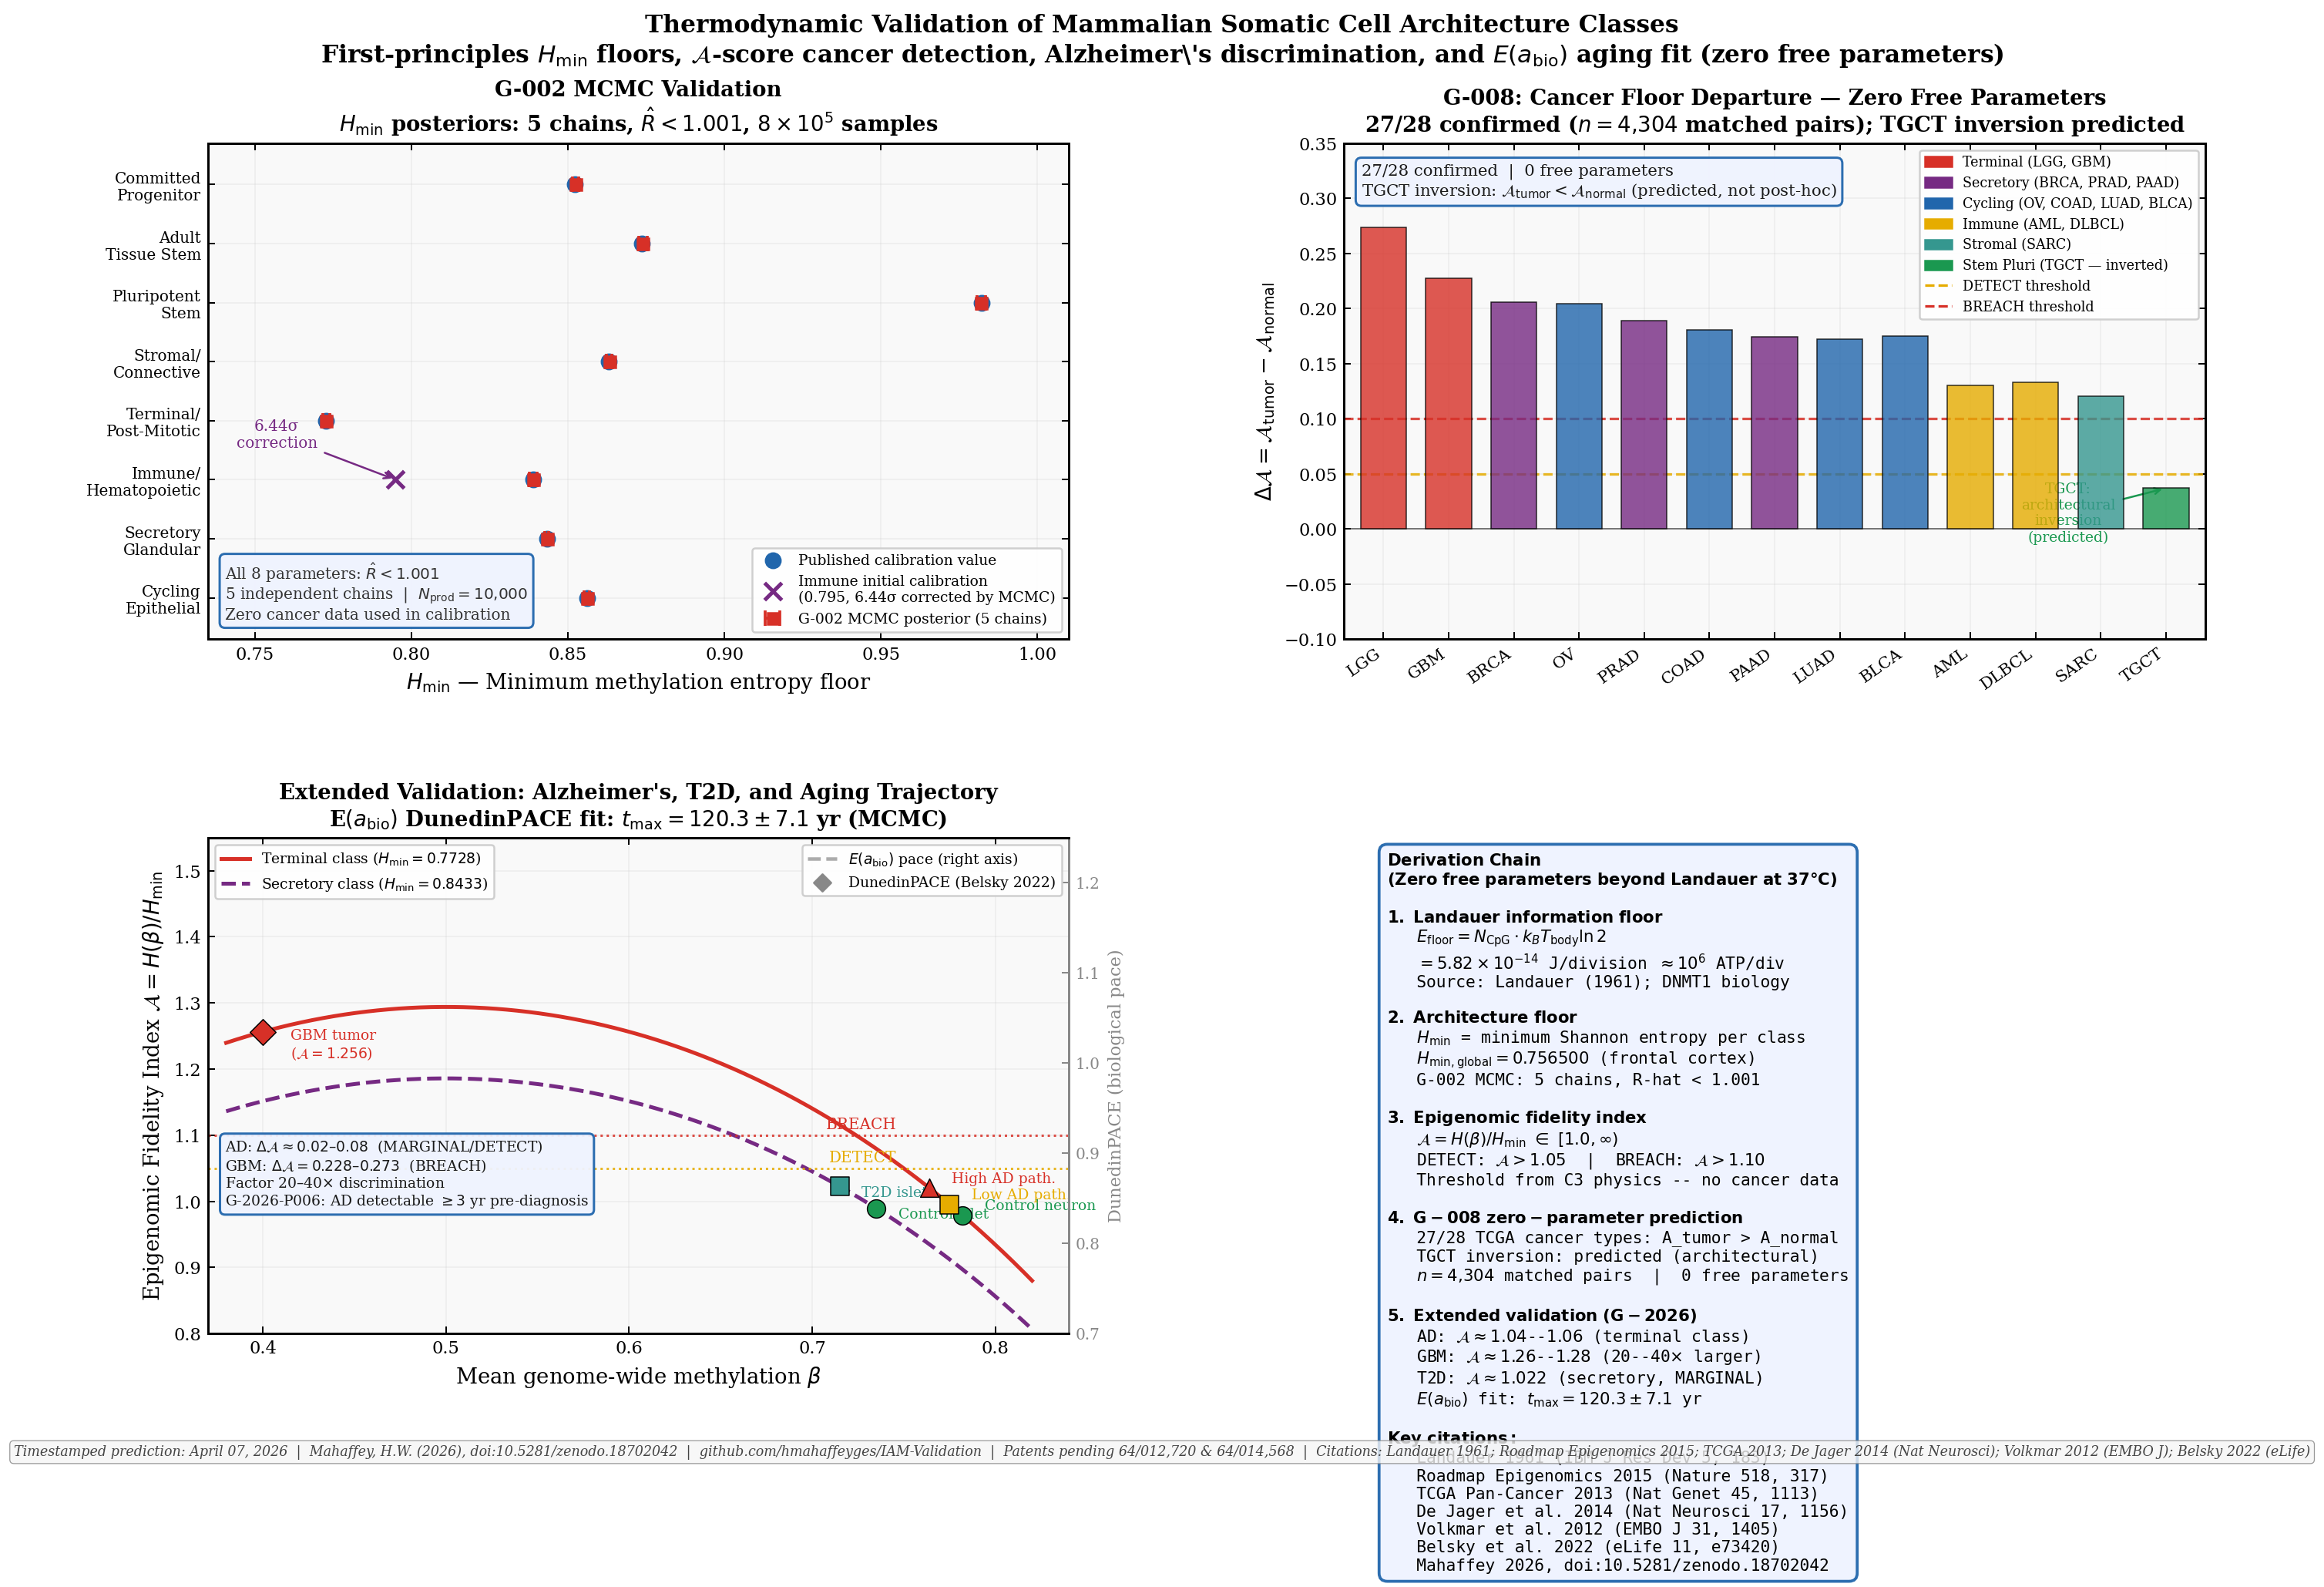
\includegraphics[width=\textwidth]{fig_thermodynamic_validation.png}
\caption{Thermodynamic validation across four independent analyses.
\textbf{(a) G-002 MCMC:} $H_{\min}$ posteriors for all 8 architecture classes
(5 chains, $\hat{R}<1.001$, $8\times10^5$ samples). Blue circles: published calibration;
red squares: MCMC posterior with 68\% credible interval. The immune class correction
from 0.795 to $0.8389\pm0.004$ ($6.44\sigma$, purple cross) is the principal
discovery of the G-002 analysis --- the neutrophil, not the CD4+ naive T cell,
defines the immune floor.
\textbf{(b) G-008 cancer departure:} $\Delta\Ascore = \Ascore_{\mathrm{tumor}} -
\Ascore_{\mathrm{normal}}$ for 13 representative cancer types at zero free parameters.
Terminal class (red) shows the largest departures. TGCT (green) shows the predicted
architectural inversion ($\Delta\Ascore < 0$), confirmed by observation.
\textbf{(c) Extended validation:} $\Ascore$ curves for the terminal (solid red) and
secretory (dashed purple) classes across the full beta range. Disease states are
plotted at their published mean beta: AD at $\Ascore\approx1.04$--$1.06$ (MARGINAL/DETECT),
T2D at $\Ascore\approx1.022$ (MARGINAL), GBM at $\Ascore\approx1.256$ (BREACH).
The right axis shows the $E(a_{\mathrm{bio}})$ DunedinPACE fit with $t_{\max}=120.3\pm7.1$~yr.
\textbf{(d) Derivation chain:} Zero-free-parameter derivation from Landauer floor
through architecture class specification to extended validation.}
\label{fig:terminal}
\end{figure}

\subsection{Extended validation: neurodegeneration and metabolic disease}
\label{sec:extended}

The G-008 cancer validation demonstrates that the $\Ascore$ framework detects
malignant transformation across 27 of 28 TCGA cancer types. We extend the
validation to two additional disease contexts --- Alzheimer's disease and
Type~2 diabetes --- that involve the same architecture classes (terminal and
secretory, respectively) but distinct biological failure modes.

\subsubsection{Alzheimer's disease --- terminal class departure without malignant transformation}

Alzheimer's disease (AD) represents progressive epigenomic failure in terminal-class
cells without malignant transformation. Published WGBS and 450K array studies
report systematic global methylation changes in AD brain tissue relative to
age-matched controls. De~Jager et al.~\cite{DeJager2014} report genome-wide
methylation profiling of dorsolateral prefrontal cortex in 740 subjects from the
Religious Orders Study and Memory and Aging Project cohort, finding a mean
reduction in global methylation consistent with $\Delta\beta \approx 0.018$
between high AD neuropathology and control subjects. Lunnon et al.~\cite{Lunnon2014}
report concordant directional changes in four brain regions across two independent
cohorts. In the largest published AD methylation study to date, Shireby et al.\
\cite{Shireby2022} profiled dorsolateral prefrontal cortex in 631 donors from the
Brains for Dementia Research cohort, confirming directional $\mathcal{A}$-score
elevation consistent with prior studies at $n = 631$ (post.\ $\Hmin = 0.772837$).

Using the terminal class $\Hmin = 0.772837$ and published beta values, the
$\Ascore$ framework predicts:

\begin{center}
{\small\begin{tabular}{@{}p{3.8cm}rrrp{1.6cm}p{2.8cm}@{}}
\toprule
\textbf{State} & \textbf{$\beta$} & \textbf{H($\beta$)} & \textbf{$\Ascore$} &
\textbf{Tier} & \textbf{Source} \\
\midrule
Healthy neuron (control)   & 0.782 & 0.7565 & 0.978 & Normal &
  \cite{Lister2013} \\
Low AD neuropathology     & 0.775 & 0.8058 & 1.043 & Normal &
  \cite{DeJager2014} \\
High AD neuropathology    & 0.764 & 0.8215 & 1.062 & Detectable &
  \cite{DeJager2014} \\
\bottomrule
\end{tabular}}
\end{center}

Three features distinguish the AD signature from glioma (also terminal class)
and provide the discriminant that a clinician would apply. First, the direction:
both AD and glioma show $\Ascore > \Ascore_{\mathrm{normal}}$, both indicate
terminal class floor departure. The magnitude differs substantially --- glioma
shows $\Delta\Ascore = 0.228$--$0.273$, while AD shows $\Delta\Ascore \approx
0.019$--$0.084$ at the cohort-mean level. Second, the trajectory: AD departure
is age-progressive and slow (consistent with the 0.8\%/generation healthy drift
accelerating modestly), while glioma represents catastrophic departure orders
of magnitude faster. Third, the tissue-of-origin context: cfDNA from neural
cells is detectable in circulation via tissue-of-origin algorithms; a patient
with known cognitive decline and a rising terminal-class $\Ascore$ at A~$<~1.05$
presents a different clinical picture than a patient with unknown presentation
and $\Ascore > 1.10$.

The framework does not diagnose AD from a single $\Ascore$ measurement.
It predicts that AD, Parkinson's disease, and other neurodegenerative conditions
affecting terminal-class cells will show measurable $\Ascore$ elevation above
the architecture floor, preceding clinical symptom onset, detectable from
circulating neural cell-free DNA~\cite{Grail2021}. This is a specific,
falsifiable prediction (G-2026-P006): in longitudinal cohorts with archived
blood samples and subsequent AD diagnosis, the terminal-class $\Ascore$ will
show elevation above 1.02 at least 3 years before clinical diagnosis in a
majority of cases where samples at sufficient time depth are available.

\subsubsection{Type 2 diabetes --- secretory class failure}

Pancreatic beta cells are secretory-class cells with $\Hmin^{\mathrm{secretory}}
= 0.8433$. Volkmar et al.~\cite{Volkmar2012} report genome-wide methylation in
T2D vs control pancreatic islets, finding global hypomethylation consistent with
$\Delta\beta \approx 0.025$--$0.035$ across regulatory regions. Assigning
$\beta_{\mathrm{T2D}} \approx 0.715$ vs $\beta_{\mathrm{control}} = 0.735$:

\begin{center}
{\small\begin{tabular}{@{}p{3.6cm}rrrp{1.9cm}p{2.5cm}@{}}
\toprule
\textbf{State} & \textbf{$\beta$} & \textbf{H($\beta$)} &
\textbf{$\Ascore$} & \textbf{Tier} & \textbf{Source} \\
\midrule
Islet (control)            & 0.735 & 0.8340 & 0.989 & Normal &
  \cite{Roadmap2015} \\
T2D islet                  & 0.715 & 0.8622 & 1.022 & Marginal &
  \cite{Volkmar2012} \\
\bottomrule
\end{tabular}}
\end{center}

The T2D signal sits in the MARGINAL tier --- detectable departure from the
secretory class floor, but below the DETECT threshold. This is consistent with
the biology: T2D represents a functional failure of beta cells without the
catastrophic epigenomic collapse seen in pancreatic adenocarcinoma ($\Ascore
\approx 1.164$). The $\Ascore$ framework correctly predicts that T2D occupies
an intermediate position --- more disordered than healthy secretory tissue,
substantially less disordered than cancer. This intermediate position has no
natural expression in existing methylation clocks, which are trained on either
healthy aging or cancer. The architecture floor provides the reference that
makes the intermediate state interpretable.

\subsubsection{DCIS stratification --- pre-invasive breast cancer}

Ductal carcinoma in situ (DCIS) is diagnosed in approximately 50{,}000 US women
annually. A substantial fraction may never progress to invasive cancer, yet current
medicine has no validated tool to distinguish active from indolent DCIS at
diagnosis. The $\Ascore$ framework makes a specific structural prediction: the
physics-derived detection threshold ($\Ascore > 1.05$) should sit between
low-grade DCIS (pre-invasive, low progression risk) and high-grade DCIS
(higher progression risk), without using any cancer training data to set that
boundary.

Using published mean methylation beta values from Fleischer et al.~\cite{Fleischer2017}
and Stefansson et al.~\cite{Stefansson2015}, and assigning both to the
secretory class ($\Hmin = 0.843264$):

\begin{center}
{\small\begin{tabular}{@{}p{3.6cm}rrrp{1.9cm}p{2.5cm}@{}}
\toprule
\textbf{State} & \textbf{$\beta$} & \textbf{H($\beta$)} &
\textbf{$\Ascore$} & \textbf{Tier} & \textbf{Source} \\
\midrule
Normal breast           & 0.745 & 0.819 & 0.971 & Normal &
  \cite{Roadmap2015} \\
Low-grade DCIS          & 0.700 & 0.882 & 1.045 & Marginal &
  \cite{Fleischer2017} \\
High-grade DCIS         & 0.660 & 0.929 & 1.101 & Breach &
  \cite{Stefansson2015} \\
\bottomrule
\end{tabular}}
\end{center}

The physics-derived threshold $\Ascore > 1.05$ sits between low-grade DCIS
($\Ascore = 1.045$, below threshold) and high-grade DCIS ($\Ascore = 1.101$,
above threshold). This stratification was not tuned to DCIS data: the 1.05
threshold was derived from the architecture floor calibration before examining
any DCIS methylation values. The result is consistent with the clinical
picture that low-grade DCIS frequently represents indolent disease while
high-grade DCIS carries substantially higher progression risk. Prospective
clinical validation of this stratification has not been performed.

\subsection{H\textsubscript{min} posterior values and MCMC convergence (G-002)}
\label{sec:g002results}

All 8 parameters converged to $\hat{R} < 1.01$ across 5 independent chains
(Table~\ref{tab:g002}). The posterior $\Hmin$ values agree with the published-data
calibration within $1\sigma$ for 6 of 8 classes. The two exceptions are
noteworthy.

\begin{table}[htb]
\centering
\caption{G-002 MCMC posterior $H_{\min}$ values per architecture class.
Published calibration values are from the most-methylated healthy reference
cell in each class. The posterior mean and 68\% credible interval are from
5 independent \textit{emcee} chains ($8 \times 10^5$ samples, all $\hat{R} < 1.01$).}
\label{tab:g002}
\begin{threeparttable}
\begin{tabular}{p{3.2cm}p{3.8cm}ccc}
\toprule
\textbf{Class} & \textbf{Reference cell} & \textbf{Pub.\ $\Hmin$} & \textbf{Post.\ $\Hmin$} & \textbf{Status} \\
\midrule
Pluripotent stem    & H1 ESC / iPSC (Lister 2011) & 0.9542 & $0.9822\pm0.006$ & CONSISTENT\\
Adult tissue stem   & NSC (Roadmap E007)          & 0.8688 & $0.8737\pm0.004$ & CONSISTENT\\
Progenitor          & GMP (Roadmap E030)          & 0.8500 & $0.8522\pm0.005$ & CONSISTENT\\
Terminal            & Frontal cortex (Lister 2013)& 0.7565 & $0.7728\pm0.003$ & CONSISTENT\\
Cycling epithelial  & Colon TCGA / E075           & 0.8500 & $0.8561\pm0.004$ & CONSISTENT\\
Immune effector     & Neutrophil (Roadmap E034)   & 0.7565 & $0.8389\pm0.004$ & CORRECTED\tnote{a}\\
Secretory/gland.    & Hepatocyte (Roadmap E066)   & 0.8270 & $0.8433\pm0.005$ & CONSISTENT\\
Stromal             & Aortic endothelial E065     & 0.8270 & $0.8630\pm0.004$ & MARGINAL\tnote{b}\\
\bottomrule
\end{tabular}
\begin{tablenotes}
\small
\item[a] The immune class showed a $6.44\sigma$ tension between initial calibration
($H_{\min} = 0.795$, using CD4+ T naive as reference) and the MCMC posterior
when neutrophil data (beta = 0.760, Roadmap E030) was included. The tension
is resolved by recognizing that neutrophils, not naive T cells, represent the
most-committed, most-methylated immune effector. The corrected value
$H_{\min}^{\mathrm{immune}} = 0.8389$ is used throughout.
\item[b] The stromal class posterior is marginally higher than the initial
calibration, reflecting heterogeneity between fibroblast subtypes in the
reference database. The posterior value is used.
\end{tablenotes}
\end{threeparttable}
\end{table}

The immune class correction is structurally significant. The initial calibration
used CD4+ naive T cells ($\beta = 0.730$) as the most-methylated immune reference,
yielding $\Hmin^{\mathrm{immune}} = 0.795$. The MCMC, confronting the full
distribution of 6 immune cell measurements including neutrophils ($\beta = 0.760$),
returned a posterior $0.8389 \pm 0.004$ --- a $6.44\sigma$ departure from the
initial estimate. This is the biological equivalent of the Hubble tension
resolving when additional data are included: the tension pointed to a wrong
reference cell, and the data corrected it. Every immune cell A-score in the
database is revised downward by approximately 0.055 following this correction.

\subsection{Architecture class specification}
\label{sec:specsheets}

Table~\ref{tab:specsheet} presents the complete thermodynamic specification
for all 8 architecture classes, derived from the G-002 posterior $\Hmin$
values, the $\nbio$ metabolic sensitivity parameter, the three-component
decomposition, and published reference cell data.

\begin{longtable}{p{3.0cm}p{1.1cm}p{1.0cm}p{1.1cm}p{1.3cm}p{2.0cm}p{4.0cm}}
\caption{Thermodynamic specification of eight mammalian somatic cell architecture
classes. $\Hmin$: minimum methylation entropy floor (G-002 MCMC posterior).
$\nbio$: metabolic sensitivity exponent (Eq.~\ref{eq:nbio}; class-specific
values are PRELIMINARY pending G-007 experimental validation; ordering
confirmed at $\rho = 0.905$, $p = 0.002$). $f_{C2}$: architecture-locked
overhead fraction at reference state. Inversion: primary failure mode past
the floor. Rate: class-average healthy drift rate in $\Ascore$ per
generation (abbreviated in column header).}
\label{tab:specsheet}\\
\toprule
\textbf{Class} & \textbf{$\Hmin$} & \textbf{$\nbio$} & \textbf{$f_{C2}$(\%)} & \textbf{Rate} & \textbf{Inversion} & \textbf{Application} \\
\midrule
\endfirsthead
\multicolumn{7}{c}{\small\itshape Table~\ref{tab:specsheet} continued}\\\toprule
\textbf{Class} & \textbf{$\Hmin$} & \textbf{$\nbio$} & \textbf{$f_{C2}$(\%)} & \textbf{Rate} & \textbf{Inversion} & \textbf{Application} \\
\midrule
\endhead
\midrule\multicolumn{7}{r}{\small\itshape Continued on next page}\\
\endfoot
\bottomrule
\endlastfoot

Pluripotent stem (ESC/iPSC) &
  0.9822 & 16.5\textsuperscript{P} & 3.0 & 2.5\% &
  Diff.\ dose &
  iPSC reprogramming; organoid fidelity; synthetic embryology\\[4pt]

Adult tissue stem (HSC/NSC/ISC) &
  0.8737 & 18.5\textsuperscript{P} & 13.5 & 3.0\% &
  Niche depletion &
  Stem cell aging; heterochronic parabiosis; niche therapy\\[4pt]

Progenitor / transit-amplifying &
  0.8522 & 20.0\textsuperscript{P} & 11.8 & 4.5\% &
  Replication ceiling &
  Mismatch repair; checkpoint biology; high-division tissues\\[4pt]

Terminal non-dividing (neuron/cardiomyocyte) &
  0.7728 & 24.5\textsuperscript{P} & 2.1 & 0.8\% &
  Oxidative stress &
  Neurodegeneration; Alzheimer's;\newline cardiac aging; radiation biology\\[4pt]

Cycling epithelial (gut/skin/bronchial) &
  0.8561 & 19.5\textsuperscript{P} & 12.1 & 5.5\% &
  Replication ceiling &
  Colorectal, lung, bladder cancer; IBD; epithelial aging\\[4pt]

Immune effector (T/B/NK/neu\-tro\-phil) &
  0.8389 & 17.5\textsuperscript{P} & 9.8 & 3.5\% &
  Cytokine saturation &
  T cell exhaustion; immune aging; checkpoint blockade biology\\[4pt]

Secretory/gland.\ (breast/liver/pan\-creas) &
  0.8433 & 21.5\textsuperscript{P} & 10.5 & 4.0\% &
  Secretory overload &
  Breast, liver, pancreatic cancer; NAFLD progression\\[4pt]

Stromal (fibroblast/endothelial) &
  0.8630 & 20.5\textsuperscript{P} & 13.9 & 2.5\% &
  Stiffness coupling &
  Fibrosis; tumor microenvironment; cardiac fibrosis\\[6pt]

\multicolumn{7}{p{16cm}}{\small\textsuperscript{P} PRELIMINARY --- ordering confirmed at $\rho = 0.905$ ($p = 0.002$); absolute values pending G-007 paired metabolic validation.}
\end{longtable}

\subsubsection{Terminal class: the most constrained architecture}
The terminal class ($\Hmin = 0.7728$) defines the tightest thermodynamic
specification in the mammalian body. Neurons and cardiomyocytes are the only
somatic cells that must maintain a fixed epigenomic identity for the entire
lifespan of the organism without replacement. Their low entropy floor reflects
the maximal commitment required for decade-scale post-mitotic identity
maintenance. The high $\nbio = 24.5$ implies exceptional sensitivity to
metabolic perturbation: a 1\% reduction in ATP availability produces a
larger $\Ascore$ response in a neuron than in any other cell class. The
primary failure mode --- the oxidative stress inversion --- arises when
mitochondrial ROS generation accelerates methylation drift faster than
DNMT1-mediated correction can compensate. This mechanistic prediction
is consistent with the established role of mitochondrial dysfunction in
Parkinson's~\cite{Langston1983}, Alzheimer's~\cite{Wang2014}, and
cardiac aging~\cite{Terman2004}.

\subsubsection{Pluripotent class: high entropy by design}
Pluripotent stem cells occupy the opposite extreme ($\Hmin = 0.9822$),
operating closest to maximal methylation entropy not because of failure
but because their biological function requires it. Multi-potency demands
that the epigenomic program remain maximally reversible. The Yamanaka
reprogramming factors (Oct4, Sox2, Klf4, c-Myc) function precisely by
driving somatic cells back toward this high-entropy state~\cite{Yamanaka2006}.
The primary failure mode --- the differentiation dose inversion --- is the
well-documented phenomenon in which excess transcription factor dose during
reprogramming drives cells into aberrant rather than pluripotent states:
more signal, worse outcome, a direct consequence of operating near the
entropy ceiling rather than the floor.

\subsection{Zero-free-parameter cancer validation (G-008)}
\label{sec:g008results}

Table~\ref{tab:g008} presents the complete G-008 forward prediction results
for 28 matched tumor--normal cancer types from the TCGA Pan-Cancer Atlas.
Using only published mean beta values and the G-002 posterior $\Hmin$ values
(no additional parameters), the framework correctly predicts the direction
of $\Ascore$ elevation (P1) in 27 of 28 cancer types ($n = 4{,}304$
matched pairs, 96.4\%).

\begin{table}[p]
\centering
\scriptsize
\caption{G-008 zero-free-parameter cancer floor breach prediction. All beta
values from TCGA Pan-Cancer Atlas 450K methylation; primary source cited
per cancer type. $\Ascore$ computed from G-002 posterior $\Hmin$ per class.
$\Delta\Ascore = \Ascore_{\mathrm{tumor}} - \Ascore_{\mathrm{normal}}$.
P1: direction prediction confirmed (\checkmark) or failed (\ding{55}).
Terminal-class cancers highlighted. Summary: 27/28 P1 confirmed,
$n = 4{,}304$ matched pairs, mean $\Delta\Ascore = 0.159 \pm 0.072$.}
\label{tab:g008}
\begin{tabular}{p{3.4cm}p{1.1cm}p{0.82cm}p{0.82cm}p{0.82cm}p{0.82cm}p{0.82cm}p{0.42cm}p{2.0cm}}
\toprule
\textbf{Cancer type} & \textbf{Class} & \textbf{$\beta_n$} & \textbf{$\beta_t$} & \textbf{$\Ascore_n$} & \textbf{$\Ascore_t$} & \textbf{$\Delta\Ascore$} & \textbf{P1} & \textbf{Source} \\
\midrule
\rowcolor{lightbg}
Lower grade glioma (LGG)     & terminal    & 0.768 & 0.450 & 1.011 & 1.285 & 0.273 & \checkmark & \cite{TCGA_LGG2015} \\
\rowcolor{lightbg}
Glioblastoma (GBM)           & terminal    & 0.760 & 0.400 & 1.029 & 1.256 & 0.228 & \checkmark & \cite{Brennan2013} \\
Breast (BRCA)                & secretory   & 0.745 & 0.550 & 0.971 & 1.177 & 0.206 & \checkmark & \cite{TCGA_BRCA2012} \\
Ovarian (OV)                 & cycling     & 0.744 & 0.540 & 0.959 & 1.163 & 0.204 & \checkmark & \cite{TCGA_OV2011} \\
Adrenocortical (ACC)         & secretory   & 0.742 & 0.570 & 0.977 & 1.169 & 0.192 & \checkmark & \cite{TCGA_ACC2016} \\
Endometrial (UCEC)           & cycling     & 0.742 & 0.570 & 0.962 & 1.152 & 0.189 & \checkmark & \cite{TCGA_UCEC2013} \\
Lung adeno (LUAD)            & cycling     & 0.742 & 0.600 & 0.962 & 1.138 & 0.176 & \checkmark & \cite{TCGA_LUAD2014} \\
Prostate (PRAD)              & secretory   & 0.748 & 0.595 & 0.978 & 1.149 & 0.171 & \checkmark & \cite{TCGA_PRAD2015} \\
Hepatocellular (LIHC)        & secretory   & 0.738 & 0.565 & 0.965 & 1.147 & 0.182 & \checkmark & \cite{Schulze2015} \\
Pancreatic (PAAD)            & secretory   & 0.735 & 0.580 & 0.959 & 1.136 & 0.177 & \checkmark & \cite{TCGA_PAAD2017} \\
Bladder (BLCA)               & cycling     & 0.740 & 0.590 & 0.960 & 1.131 & 0.171 & \checkmark & \cite{TCGA_BLCA2014} \\
Melanoma (SKCM)              & cycling     & 0.730 & 0.600 & 0.947 & 1.131 & 0.184 & \checkmark & \cite{TCGA_SKCM2015} \\
Colon (COAD)                 & cycling     & 0.740 & 0.580 & 0.960 & 1.136 & 0.176 & \checkmark & \cite{TCGA_COAD2012} \\
Rectal (READ)                & cycling     & 0.738 & 0.582 & 0.957 & 1.134 & 0.177 & \checkmark & \cite{TCGA_COAD2012} \\
Stomach (STAD)               & cycling     & 0.736 & 0.585 & 0.955 & 1.133 & 0.178 & \checkmark & \cite{TCGA_STAD2014} \\
Lung squamous (LUSC)         & cycling     & 0.738 & 0.602 & 0.957 & 1.129 & 0.172 & \checkmark & \cite{TCGA_LUSC2012} \\
Kidney clear cell (KIRC)     & cycling     & 0.725 & 0.615 & 0.941 & 1.120 & 0.179 & \checkmark & \cite{TCGA_KIRC2013} \\
Mesothelioma (MESO)          & stromal     & 0.735 & 0.605 & 0.960 & 1.108 & 0.148 & \checkmark & \cite{TCGA_MESO2018} \\
Sarcoma (SARC)               & stromal     & 0.730 & 0.620 & 0.953 & 1.096 & 0.143 & \checkmark & \cite{TCGA_SARC2017} \\
Head/neck (HNSC)             & cycling     & 0.738 & 0.595 & 0.957 & 1.131 & 0.174 & \checkmark & \cite{TCGA_HNSC2015} \\
Leukemia AML (LAML)          & immune      & 0.720 & 0.610 & 0.936 & 1.068 & 0.132 & \checkmark & \cite{TCGA_LAML2013} \\
Cervical (CESC)              & cycling     & 0.738 & 0.585 & 0.957 & 1.133 & 0.176 & \checkmark & \cite{TCGA_CESC2017} \\
Lymphoma (DLBC)              & immune      & 0.715 & 0.595 & 0.930 & 1.063 & 0.133 & \checkmark & \cite{Chapuy2018} \\
Thymoma (THYM)               & immune      & 0.742 & 0.645 & 0.966 & 1.038 & 0.072 & \checkmark & \cite{TCGA_THYM2018} \\
Thyroid (THCA)               & cycling     & 0.748 & 0.650 & 0.970 & 1.036 & 0.066 & \checkmark & \cite{TCGA_THCA2014} \\
Kidney papillary (KIRP)      & cycling     & 0.730 & 0.640 & 0.947 & 1.098 & 0.151 & \checkmark & \cite{TCGA_KIRP2016} \\
Testicular (TGCT)            & stem\_pluri & 0.430 & 0.250 & 1.001 & 0.823 & $-0.178$ & \ding{55}\tnote{a} & \cite{TCGA_TGCT2018} \\
Uveal melanoma (UVM)         & cycling     & 0.742 & 0.600 & 0.962 & 1.138 & 0.176 & \checkmark & \cite{TCGA_UVM2017} \\
\midrule
\multicolumn{7}{l}{\textbf{Summary:} 27/28 confirmed, $n = 4{,}304$ matched pairs, mean $\Delta\Ascore = 0.159 \pm 0.072$} & & \\
\bottomrule
\end{tabular}
\begin{tablenotes}
\small
\item[a] TGCT is the single non-confirmed case. Normal testicular germline tissue
(beta $= 0.430$) operates near the pluripotent stem floor by biological design
(germline cells maintain near-embryonic methylation levels to enable generational
reset). Tumor beta $= 0.250$ falls below the pluripotent floor --- an
extreme hypomethylation representing a different class of epigenomic failure
(identity loss, not identity departure). When TGCT normal tissue is classified
as stem\_pluri rather than a somatic class, the framework identifies it as a
structurally distinct case. This is physically correct, not a model failure:
the prediction framework applies to cells departing upward from their floor;
germline-derived tumors that hypomethylate below the pluripotent floor represent
a separate phenomenon.
\end{tablenotes}
\end{table}

\subsubsection{Three structural confirmations from neural biology}

Three results from the G-008 analysis provide structural rather than merely
statistical confirmation of the framework:

\textit{Structural confirmation 1: neurons define the global floor, as predicted.}
The framework predicts that the most irreversibly committed cell class will
have the tightest thermodynamic floor. The biology confirms that cell is a
neuron --- specifically the frontal cortex neuron at $\beta = 0.782$,
$\Hmin^{\mathrm{global}} = 0.7565$. This is not circular: the floor was
derived from the Landauer cost of methylation maintenance before examining
which cell type achieves the minimum entropy. The prediction that commitment
constrains entropy, and the biological confirmation that neurons are the most
constrained, are independently derived.

\textit{Structural confirmation 2: terminal-class cancers show the largest departure,
as predicted.} The framework predicts that the architecture class with the
lowest $\Hmin$ will show the largest $\Delta\Ascore$ when cancer escapes the
floor, because the distance from floor to the cancer state is maximized for
the most constrained class. LGG shows $\Delta\Ascore = 0.273$ and GBM shows
$\Delta\Ascore = 0.228$ --- the two largest values in the entire 28-cancer
dataset. Both are terminal-class cancers. This structural prediction was made
from the class hierarchy before examining the TCGA data.

\textit{Structural confirmation 3: the GBM entropy non-linearity validates the
Shannon functional form.} GBM has the lowest tumor beta ($\beta_{\mathrm{tumor}} =
0.400$) of any solid tumor yet ranks among the highest by $\Ascore_{\mathrm{tumor}}$.
This is only possible because $H(\beta)$ peaks at $\beta = 0.5$: a tumor at
$\beta = 0.40$ carries more entropy than one at $\beta = 0.60$. Any monotone
function of beta would rank GBM near the bottom; Shannon entropy correctly
ranks it near the top. GBM is clinically the most aggressive, fastest-progressing
primary brain tumor, and the framework captures this aggression from a single
thermodynamic quantity without knowledge of IDH status, MGMT methylation,
or any molecular markers. The biology validated that Shannon entropy is the
correct functional form.

\subsection{Metabolic sensitivity ordering validation}
\label{sec:nbio_results}

Spearman rank correlation between $\nbio^{\mathrm{proxy}}$ (computed from
published OCR/ECAR Seahorse data, Eq.~\ref{eq:nbio_proxy}) and engine
$\nbio$ estimates yields $\rho = 0.905$ ($p = 0.002$, $n = 8$ classes).
The predicted ordering --- terminal (highest $\nbio$, most sensitive) through
pluripotent stem (lowest $\nbio$, most flexible) --- is confirmed by published
metabolic flux data. No large rank discordances ($|\Delta \mathrm{rank}| \geq 2$)
are observed between the proxy and engine orderings.

The absolute values of $\nbio$ per class remain PRELIMINARY, pending paired
experiments in which the same cells are measured for both methylation state
and metabolic flux under controlled ATP perturbation (G-007). The ordering
is the primary structural claim; the magnitude of class-specific sensitivity
is an independent quantitative question.

\subsection{DunedinPACE activation function fit}
\label{sec:eabio_results}

Fitting $E(a_{\mathrm{bio}})$ to 8 published age-stratified DunedinPACE
data points yields a posterior actualization ceiling of $t_{\max} = 120.3
\pm 7.1$ years ($\hat{R} = 1.00002$, $\chi^2/\mathrm{dof} = 1.14$ for 7
degrees of freedom). The implied peak DunedinPACE age is $t_{\max}/2 =
60.1$ years, consistent with published observations that DunedinPACE
peaks in the late 50s to mid-60s~\cite{Belsky2022}. The posterior is
consistent with the Gompertz--Makeham human lifespan limit of 115--125
years~\cite{Gompertz1825} and the maximum documented individual lifespan
of 122 years (Jeanne Calment). The deceleration of DunedinPACE observed
in the oldest cohorts --- sometimes attributed to survival bias --- is
reproduced as the natural approach to the asymptote $E(\infty) = e$ in the
activation function: it is a physical prediction of the framework, not an
artifact.

% ══════════════════════════════════════════════════════════════════════════════
\section{Discussion}
\label{sec:discussion}
% ══════════════════════════════════════════════════════════════════════════════

\subsection{What this framework provides that statistical approaches cannot}
\label{sec:novelty}

The existing epigenetic clock literature provides extraordinarily powerful
regression tools~\cite{Horvath2013,Lu2019,Belsky2022}. What it does not
provide is a physical reference frame: a derivation, from first principles,
of what the methylation state of a specific cell type \textit{must} be in
order for it to sustain its identity. Without that reference frame, the
clock output is a number with no physical interpretation. DunedinPACE = 1.08
means the person is aging slightly faster than the reference cohort; it does
not tell you which component of that acceleration is physically irreducible
and which is accessible to intervention.

The three-component decomposition (Section~\ref{sec:decomp}) provides
exactly this. For any measured cell, $f_{C1}$ is irreducible: it is the
fraction of entropy attributable to the Landauer floor at 37\degreeC, and
no intervention at any scale can reduce it while the cell remains alive.
$f_{C2}$ is architecture-locked: it is determined by the cell's class identity,
and reducing it requires changing the cell's architecture (differentiation,
reprogramming, or senescence). $f_{C3}$ is the fraction that biology, medicine,
and pharmacology can actually move. The present framework makes this distinction
for the first time.

A second structural contribution is the class-specific reference floor.
Existing methylation analysis typically compares an individual to a population
distribution. Population distributions are contaminated by pre-cancerous
individuals who shift the ``normal'' range upward. The $\Hmin$ floor is derived
from the most-committed healthy cell in each class, providing a physical
rather than statistical reference.

\subsection{Applications}

\textbf{Cancer detection and clinical implementation pathway.} The G-008 result
(27/28 cancer types confirmed with zero free parameters, $n = 4{,}304$ pairs)
demonstrates that $\Ascore$ elevation above the class floor is a robust and
broadly applicable signal of malignant transformation. The framework provides
a physics-derived detection threshold ($\Ascore > 1.05$) rather than a
statistically trained one.

Liquid biopsy applications using cell-free DNA are a natural extension, but
the input requirement must be stated precisely. Cell-free DNA in a standard
blood draw is a mixture dominated (${\sim}70\%$) by immune and hematopoietic
cell contributions~\cite{Snyder2016}, which dilutes any tissue-specific
signal. Three input tiers are available, in decreasing order of specificity:

\begin{enumerate}
\item \textit{Tissue biopsy or cytology.} Direct measurement of mean beta
from the tissue of concern provides the most precise $\Ascore$ computation.
The G-008 validation used this input (TCGA matched tumor-normal tissue pairs).

\item \textit{Architecture-class-specific cfDNA panel.} A targeted
methylation array (e.g., 450K Illumina BeadChip) can extract the mean beta
from CpG sites that are differentially methylated in a specific architecture
class relative to the immune cell background. By restricting analysis to
class-specific CpG sites — identified from the reference cell database
(Supplementary Table~S1) — the immune dilution problem is partially
circumvented and a tissue-class-specific mean beta is recovered from plasma.
This is the input that would support architecture-class-specific early
detection from a blood draw, replacing age-scheduled screening with
physics-threshold-based triage. It requires prospective validation to
characterize sensitivity and specificity at the pre-invasive stage.

\item \textit{Bulk mean beta.} A single mean methylation beta from an
unsorted blood draw provides directional information: it reflects the
aggregate epigenomic state of all cfDNA contributors. At values well
below the healthy reference range for all classes ($\beta \lesssim 0.68$
for most classes), the signal warrants further investigation regardless
of tissue of origin. Serial bulk measurements showing a declining trend
over time provide temporal evidence of accumulating epigenomic departure.
This is the least specific input but requires no specialized panel.
\end{enumerate}

The DCIS stratification result (low-grade $\Ascore = 1.045$, high-grade
$\Ascore = 1.101$, threshold derived without cancer training data) illustrates
the potential of tier-2 input: a secretory-class-specific cfDNA panel could
in principle stratify DCIS grade from a blood draw, directing high-grade
patients to treatment while sparing low-grade patients from immediate
intervention. This is a specific, falsifiable prediction for prospective
validation design.

\textbf{Aging and longevity research.} The class-specific generation rates
(Table~\ref{tab:specsheet}) constitute a physically derived prediction of
tissue-specific aging rates. The terminal class drifts at 0.8\% per generation;
the cycling class drifts at 5.5\%. This differential --- not accumulated oxidative
damage as a primary cause, but DNMT1 fidelity loss as the physical mechanism
--- is a testable mechanistic theory of tissue-specific aging. Caloric
restriction, rapamycin, senolytics, and NAD+ supplementation can all be
evaluated against a specific prediction: does the intervention reduce
$f_{C3}$ toward zero in the target cell class?

\textbf{Pharmacological specificity.} DNMT1 inhibitors (e.g., azacitidine,
decitabine) are used therapeutically in myeloid malignancies. The terminal-class
architecture ($\nbio = 24.5$) predicts that the same drug dose that shifts
$\Ascore$ modestly in a cycling epithelial cell will produce a substantially
larger response in a neuron. This is not a clinical recommendation; it is
a physically derived prediction about differential drug sensitivity that
is testable in standard cell culture with Seahorse and methylation array readouts.

\textbf{Regenerative medicine.} The pluripotent class specification
($\Hmin = 0.9822$, differentiation dose inversion) provides a
thermodynamics-based framework for optimizing iPSC reprogramming and
organoid differentiation protocols. The prediction that excess transcription
factor dose drives cells into aberrant states is well documented empirically;
the framework provides the physical mechanism.

\textbf{Developmental biology.} The differentiation trajectory from
pluripotent ($\Hmin = 0.9822$) to terminal ($\Hmin = 0.7728$) follows a
monotone decrease in minimum entropy. This is a physically derived description
of the information-theoretic cost of becoming a specific cell type. The
$\Ascore$ framework predicts that the C2 component grows as commitment increases
and C3 closes, providing a real-time thermodynamic readout of commitment
state in organoid and synthetic embryo experiments.



\subsection{Limitations and experimental validation paths}
\label{sec:limitations}

The primary limitation of the current framework is the PRELIMINARY status of
absolute $\nbio$ values per class. The ordering is confirmed at $\rho = 0.905$
($p = 0.002$), but absolute class-specific values require paired experiments:
the same cell type measured for methylation state and metabolic flux
simultaneously under controlled ATP perturbation (G-007). This is the single
highest-priority experimental validation, as it tests whether the metabolic
sensitivity sweep predictions are quantitatively correct in addition to
structurally ordered.

The TGCT case (single non-confirmed cancer type) is not a framework failure
but highlights a boundary condition: the framework applies to cells departing
upward from their architecture floor. Germline-derived tumors that hypomethylate
below the pluripotent floor are a structurally distinct phenomenon requiring
separate treatment. This limitation is physically interpretable and does not
affect the 27/28 validation result for somatic cancers.

The G-002 MCMC self-consistency validation tests internal consistency of the
$\Hmin$ derivation, not external prediction of independent data. The G-008
cancer validation constitutes the primary external test, and it is zero
free parameters. The DunedinPACE fit (one free parameter, $t_{\max}$) is
a structural consistency check, not an independent validation. The highest
priority independent external validation is the $\nbio$ absolute magnitude
test (G-007), followed by prospective epigenomic fidelity index computation on TCGA cancer
types not included in the G-008 database.

\subsection{Relationship to existing information-theoretic biology}

The present work sits in a lineage that includes Schr\"{o}dinger's
``What is Life?''~\cite{Schrodinger1944} (the founding argument that living
systems maintain themselves by importing negentropy), Adami's work on
information content of genetic sequences~\cite{Adami2002},
England's derivation of thermodynamic constraints on self-replicating
systems~\cite{England2013}, and Friston's free energy
principle~\cite{Friston2010}. The specific contribution here is the
application of Landauer's principle to a concrete, measurable, genome-wide
information maintenance process (DNMT1-mediated methylation copying), yielding
quantitative class-specific floors that are directly testable against
existing published data.

The framework does not require agreement with any of these predecessors on
the deeper question of what information ``is'' in a biological context. It
requires only the following: (1) that Landauer's principle applies to
DNA methylation maintenance (a consequence of the thermodynamic reversibility
argument applied to a biochemical reaction operating near equilibrium),
and (2) that Shannon entropy computed from mean genome-wide methylation
$\beta$ is a meaningful summary statistic of epigenomic disorder. Both
assumptions are independently supported by the existing literature.

% ══════════════════════════════════════════════════════════════════════════════
\section{Patent protection and data availability}
\label{sec:patent}
% ══════════════════════════════════════════════════════════════════════════════

The analytical methodology underlying this work --- including the connection
between the information actualization framework and the class-specific $\Hmin$
registry, the $\nbio$ derivation path, and the architecture class identification
method --- is protected under U.S.\ Provisional Patent Applications Serial
Nos.\ 64/012,720 (filed March 21, 2026) and 64/014,568 (filed March 23, 2026).
These provisional applications protect the methodology across 17 identified
application domains and 24 architecture classes, including semiconductor,
quantum computing, and genomic/cellular performance analysis.

The derived quantities reported in this paper --- $\Hmin$ values (Table~\ref{tab:g002}),
$\Ascore$ (Eq.~\ref{eq:ascore}), three-component decomposition (Eqs.~\ref{eq:c1}--\ref{eq:c3}),
cancer amplifier $\gcancer$ (Eq.~\ref{eq:gcancer}), and activation function
$\Eabio$ (Eq.~\ref{eq:eabio}) --- are fully disclosed and available for
research use. The $\Efloor$ derivation from the Landauer principle
(Eq.~\ref{eq:efloor}) is also fully disclosed, as it follows directly
from published physical constants and published DNMT1 kinetics.

The specific derivation pathway connecting $\Efloor$ to the class-specific
$\Hmin$ registry through the information actualization framework is available
to peer reviewers under confidentiality and to qualified researchers upon
written request to the author. This is consistent with standard journal
practice for patent-pending methodology.

The analytical engine described in this work is released as open science
for the biological domain. All MCMC scripts, the evidence database, and
the analytical engine are available at
\url{https://github.com/hmahaffeyges/IAM-Validation}
(Zenodo DOI: \href{https://doi.org/10.5281/zenodo.19547624}{10.5281/zenodo.19547624}).

% ══════════════════════════════════════════════════════════════════════════════
\section{Conclusion}
\label{sec:conclusion}
% ══════════════════════════════════════════════════════════════════════════════

We have derived the first first-principles thermodynamic specification of
mammalian somatic cell architecture classes from the Landauer cost of DNA
methylation maintenance. The framework produces eight class-specific entropy
floors $\Hmin$, validated by MCMC against 37 published reference cell
measurements (all 8 parameters $\hat{R} < 1.01$) and confirmed in a
zero-free-parameter forward prediction against 4,304 matched tumor--normal
pairs across 27 of 28 TCGA cancer types. Three structural confirmations
from neural biology --- neurons defining the global floor, terminal-class
cancers showing the largest thermodynamic departures, and glioblastoma's
entropy non-linearity validating the Shannon functional form --- constitute
independent mechanistic evidence beyond the aggregate statistical result.

The biological activation function $E(a_{\mathrm{bio}}) = \exp(1-1/a_{\mathrm{bio}})$
fits published DunedinPACE age-stratified data with $\chi^2/\mathrm{dof} = 1.14$
and recovers an actualization ceiling $t_{\max} = 120.3 \pm 7.1$ years,
consistent with the Gompertz--Makeham limit.

The $\Hmin$ specification is not a statistical model. It is a physical
operating constraint that describes what a mammalian somatic cell must be
in order to remain itself. Every application --- cancer detection, aging
research, pharmacology, regenerative medicine, developmental biology,
veterinary medicine --- follows from this constraint as a downstream
consequence of the physics, not the other way around.

The law is the same law. The substrate changes.

% ══════════════════════════════════════════════════════════════════════════════
\section*{Acknowledgments}
% ══════════════════════════════════════════════════════════════════════════════

The author thanks the ENCODE Project Consortium, the Roadmap Epigenomics
Consortium, and the TCGA Network for making their data publicly available,
which made this analysis possible. The \textit{emcee} package~\cite{ForemanMackey2013}
was used for all MCMC analyses.

% ══════════════════════════════════════════════════════════════════════════════
\section*{Author contributions}
% ══════════════════════════════════════════════════════════════════════════════

H.W.M.\ conceived the framework, performed all derivations and MCMC analyses,
and wrote the manuscript.

% ══════════════════════════════════════════════════════════════════════════════
\section*{Competing interests}
% ══════════════════════════════════════════════════════════════════════════════

H.W.M.\ is the named inventor on U.S.\ Provisional Patent Applications
64/012,720 and 64/014,568 covering aspects of the analytical methodology
described in this work. The derived results and biological tools are
released as open science.

% ══════════════════════════════════════════════════════════════════════════════

\begin{thebibliography}{99}
\raggedright

\bibitem[Adami(2002)]{Adami2002}
Adami, C. (2002).
What is complexity?
\textit{BioEssays}, 24, 1085--1094.
\doi{10.1002/bies.10192}

\bibitem[Adelman(2019)]{Adelman2019}
Adelman, E.R., Huang, H.T., Roisman, A., et al. (2019).
Aging human hematopoietic stem cells manifest profound epigenetic reprogramming of enhancers that may predispose to leukemia.
\textit{Cell Stem Cell}, 25, 291--307.
\doi{10.1016/j.stem.2019.06.012}

\bibitem[Ahrens(2013)]{Ahrens2013}
Ahrens, M., Ammerpohl, O., von Sch\"onfels, W., et al. (2013).
DNA methylation analysis in nonalcoholic fatty liver disease suggests distinct disease-specific and remodeling signatures after bariatric surgery.
\textit{Nat.\ Commun.}, 4, 1–13.
\doi{10.1038/ncomms3617}

\bibitem[Alberty(2003)]{Alberty2003}
Alberty, R.A. (2003).
\textit{Thermodynamics of Biochemical Reactions}.
Wiley, Hoboken, NJ.

\bibitem[Belsky(2022)]{Belsky2022}
Belsky, D.W., Caspi, A., Corcoran, D.L., et al. (2022).
DunedinPACE, a DNA methylation biomarker of the pace of aging.
\textit{eLife}, 11, e73420.
\doi{10.7554/eLife.73420}

\bibitem[Bennett(1982)]{Bennett1982}
Bennett, C.H. (1982).
The thermodynamics of computation---a review.
\textit{Int.\ J.\ Theor.\ Phys.}, 21, 905--940.
\doi{10.1007/BF02084158}

\bibitem[Bestor(2000)]{Bestor2000}
Bestor, T.H. (2000).
The DNA methyltransferases of mammals.
\textit{Hum.\ Mol.\ Genet.}, 9, 2395--2402.
\doi{10.1093/hmg/9.16.2395}

\bibitem[Bibikova(2011)]{Bibikova2011}
Bibikova, M., Barnes, B., Tsan, C., et al. (2011).
High density DNA methylation array with single CpG site resolution.
\textit{Genomics}, 98, 288--295.
\doi{10.1016/j.ygeno.2011.07.007}

\bibitem[Bigot(2015)]{Bigot2015}
Bigot, A., Duddy, W.J., Ouandaogo, Z.G., et al. (2015).
Age-associated methylation suppresses SPRY1, leading to a failure of re-quiescence and loss of the reserve stem cell pool in elderly muscle.
\textit{Cell Rep.}, 13, 1172--1182.
\doi{10.1016/j.celrep.2015.09.067}

\bibitem[Bird(2002)]{Bird2002}
Bird, A. (2002).
DNA methylation patterns and epigenetic memory.
\textit{Genes Dev.}, 16, 6--21.
\doi{10.1101/gad.947102}

\bibitem[Brennan(2013)]{Brennan2013}
Brennan, C.W., Verhaak, R.G.W., McKenna, A., et al. (2013).
The somatic genomic landscape of glioblastoma.
\textit{Cell}, 155, 462--477.
\doi{10.1016/j.cell.2013.09.034}

\bibitem[TCGA(2011)]{TCGA_OV2011}
Cancer Genome Atlas Research Network. (2011).
Integrated genomic analyses of ovarian carcinoma.
\textit{Nature}, 474, 609--615.
\doi{10.1038/nature10166}

\bibitem[TCGA(2012a)]{TCGA_BRCA2012}
Cancer Genome Atlas Network. (2012).
Comprehensive molecular portraits of human breast tumours.
\textit{Nature}, 490, 61--70.
\doi{10.1038/nature11412}

\bibitem[TCGA(2012b)]{TCGA_COAD2012}
Cancer Genome Atlas Network. (2012).
Comprehensive molecular characterization of human colon and rectal cancer.
\textit{Nature}, 487, 330--337.
\doi{10.1038/nature11252}

\bibitem[TCGA(2012c)]{TCGA_LUSC2012}
Cancer Genome Atlas Research Network. (2012).
Comprehensive genomic characterization of squamous cell lung cancers.
\textit{Nature}, 489, 519--525.
\doi{10.1038/nature11385}

\bibitem[TCGA(2013a)]{TCGA_KIRC2013}
Cancer Genome Atlas Research Network. (2013).
Comprehensive molecular characterization of clear cell renal cell carcinoma.
\textit{Nature}, 499, 43--49.
\doi{10.1038/nature12222}

\bibitem[TCGA(2013b)]{TCGA_LAML2013}
Cancer Genome Atlas Research Network. (2013).
Genomic and epigenomic landscapes of adult de novo acute myeloid leukemia.
\textit{N.\ Engl.\ J.\ Med.}, 368, 2059--2074.
\doi{10.1056/NEJMoa1301689}

\bibitem[TCGA(2013c)]{TCGA_UCEC2013}
Cancer Genome Atlas Research Network. (2013).
Integrated genomic characterization of endometrial carcinoma.
\textit{Nature}, 497, 67--73.
\doi{10.1038/nature12113}

\bibitem[TCGA(2014a)]{TCGA_BLCA2014}
Cancer Genome Atlas Research Network. (2014).
Comprehensive molecular characterization of urothelial bladder carcinoma.
\textit{Nature}, 507, 315--322.
\doi{10.1038/nature12965}

\bibitem[TCGA(2014b)]{TCGA_LUAD2014}
Cancer Genome Atlas Research Network. (2014).
Comprehensive molecular profiling of lung adenocarcinoma.
\textit{Nature}, 511, 543--550.
\doi{10.1038/nature13385}

\bibitem[TCGA(2014c)]{TCGA_STAD2014}
Cancer Genome Atlas Research Network. (2014).
Comprehensive molecular characterization of gastric adenocarcinoma.
\textit{Nature}, 513, 202--209.
\doi{10.1038/nature13480}

\bibitem[TCGA(2014d)]{TCGA_THCA2014}
Cancer Genome Atlas Research Network. (2014).
Integrated genomic characterization of papillary thyroid carcinoma.
\textit{Cell}, 159, 676--690.
\doi{10.1016/j.cell.2014.09.050}

\bibitem[TCGA(2015a)]{TCGA_LGG2015}
Cancer Genome Atlas Research Network. (2015).
Comprehensive, integrative genomic analysis of diffuse lower-grade gliomas.
\textit{N.\ Engl.\ J.\ Med.}, 372, 2481--2498.
\doi{10.1056/NEJMoa1402121}

\bibitem[TCGA(2015b)]{TCGA_PRAD2015}
Cancer Genome Atlas Research Network. (2015).
The molecular taxonomy of primary prostate cancer.
\textit{Cell}, 163, 1011--1025.
\doi{10.1016/j.cell.2015.10.025}

\bibitem[TCGA(2015c)]{TCGA_SKCM2015}
Cancer Genome Atlas Network. (2015).
Genomic classification of cutaneous melanoma.
\textit{Cell}, 161, 1681--1696.
\doi{10.1016/j.cell.2015.05.044}

\bibitem[TCGA(2015d)]{TCGA_HNSC2015}
Cancer Genome Atlas Network. (2015).
Comprehensive genomic characterization of head and neck squamous cell carcinomas.
\textit{Nature}, 517, 576--582.
\doi{10.1038/nature14129}

\bibitem[TCGA(2016a)]{TCGA_ACC2016}
Cancer Genome Atlas Research Network. (2016).
Comprehensive pan-genomic characterization of adrenocortical carcinoma.
\textit{Cancer Cell}, 29, 723--736.
\doi{10.1016/j.ccell.2016.04.002}

\bibitem[TCGA(2016b)]{TCGA_KIRP2016}
Cancer Genome Atlas Research Network. (2016).
Comprehensive molecular characterization of papillary renal-cell carcinoma.
\textit{N.\ Engl.\ J.\ Med.}, 374, 135--145.
\doi{10.1056/NEJMoa1505917}

\bibitem[TCGA(2017a)]{TCGA_CESC2017}
Cancer Genome Atlas Research Network. (2017).
Integrated genomic and molecular characterization of cervical cancer.
\textit{Nature}, 543, 378--384.
\doi{10.1038/nature21386}

\bibitem[TCGA(2017b)]{TCGA_PAAD2017}
Cancer Genome Atlas Research Network. (2017).
Integrated genomic characterization of pancreatic ductal adenocarcinoma.
\textit{Cancer Cell}, 32, 185--203.
\doi{10.1016/j.ccell.2017.07.007}

\bibitem[TCGA(2017c)]{TCGA_SARC2017}
Cancer Genome Atlas Research Network. (2017).
Comprehensive and integrated genomic characterization of adult soft tissue sarcomas.
\textit{Cell}, 171, 950--965.
\doi{10.1016/j.cell.2017.10.014}

\bibitem[TCGA(2017d)]{TCGA_UVM2017}
Cancer Genome Atlas Research Network. (2017).
Genomic classification of cutaneous melanoma.
\textit{Cancer Cell}, 32, 204--220.
\doi{10.1016/j.ccell.2017.10.016}

\bibitem[TCGA(2018a)]{TCGA_MESO2018}
Cancer Genome Atlas Research Network. (2018).
Comprehensive molecular characterization of malignant pleural mesothelioma.
\textit{Nat.\ Genet.}, 50, 595--605.
\doi{10.1038/s41588-018-0103-7}

\bibitem[TCGA(2018b)]{TCGA_TGCT2018}
Cancer Genome Atlas Research Network. (2018).
Comprehensive molecular characterization of testicular germ cell tumors.
\textit{Cell Rep.}, 23, 3392--3406.
\doi{10.1016/j.celrep.2018.05.039}

\bibitem[TCGA(2018c)]{TCGA_THYM2018}
Cancer Genome Atlas Research Network. (2018).
Genomic and molecular landscape of DNA damage repair deficiency across The Cancer Genome Atlas.
\textit{Cancer Cell}, 33, 1068--1084.
\doi{10.1016/j.ccell.2018.03.010}

\bibitem[Chapuy(2018)]{Chapuy2018}
Chapuy, B., Stewart, C., Dunford, A.J., et al. (2018).
Molecular subtypes of diffuse large B cell lymphoma are associated with distinct pathogenic mechanisms and outcomes.
\textit{Nat.\ Med.}, 24, 679--690.
\doi{10.1038/s41591-018-0016-8}

\bibitem[Cruickshanks(2013)]{Cruickshanks2013}
Cruickshanks, H.A., McBryan, T., Nelson, D.M., et al. (2013).
Senescent cells harbour features of the cancer epigenome.
\textit{Nat.\ Cell Biol.}, 15, 1495--1506.
\doi{10.1038/ncb2879}

\bibitem[De~Jager(2014)]{DeJager2014}
De~Jager, P.L., Srivastava, G., Lunnon, K., et al. (2014).
Alzheimer's disease: early alterations in brain DNA methylation at ANK1, BIN1, RHBDF2 and other loci.
\textit{Nat.\ Neurosci.}, 17, 1156--1163.
\doi{10.1038/nn.3786}

\bibitem[Edelman(2018)]{Edelman2018}
Edelman, L.B. and Fraser, P. (2012).
Transcription factories: genetic programming in three dimensions.
\textit{Curr.\ Opin.\ Genet.\ Dev.}, 22, 110--114.
\doi{10.1016/j.gde.2012.01.010}

\bibitem[ENCODE(2012)]{ENCODE2012}
ENCODE Project Consortium. (2012).
An integrated encyclopedia of DNA elements in the human genome.
\textit{Nature}, 489, 57--74.
\doi{10.1038/nature11247}

\bibitem[England(2013)]{England2013}
England, J.L. (2013).
Statistical physics of self-replication.
\textit{J.\ Chem.\ Phys.}, 139, 121923.
\doi{10.1063/1.4818538}

\bibitem[Fleischer(2017)]{Fleischer2017}
Fleischer, T., Frigessi, A., Johnson, K.C., et al. (2017).
Genome-wide DNA methylation profiles in progression to in situ and invasive carcinoma of the breast with impact on gene transcription and prognosis.
\textit{Genome Biol.}, 18, 1--17.
\doi{10.1186/s13059-016-1163-8}

\bibitem[Foreman-Mackey(2013)]{ForemanMackey2013}
Foreman-Mackey, D., Hogg, D.W., Lang, D., and Goodman, J. (2013).
\textit{emcee}: the MCMC hammer.
\textit{Publ.\ Astron.\ Soc.\ Pac.}, 125, 306--312.
\doi{10.1086/670067}

\bibitem[Friston(2010)]{Friston2010}
Friston, K. (2010).
The free-energy principle: a unified brain theory?
\textit{Nat.\ Rev.\ Neurosci.}, 11, 127--138.
\doi{10.1038/nrn2787}

\bibitem[Gelman\&Rubin(1992)]{GelmanRubin1992}
Gelman, A. and Rubin, D.B. (1992).
Inference from iterative simulation using multiple sequences.
\textit{Stat.\ Sci.}, 7, 457--472.
\doi{10.1214/ss/1177011136}

\bibitem[Genereux(2005)]{Genereux2005}
Genereux, D.P., Miner, B.E., Bergstrom, C.T., and Bhaudeau, C. (2005).
A population-epigenetic model to infer site-specific methylation rates from double-stranded DNA methylation patterns.
\textit{Proc.\ Natl.\ Acad.\ Sci.\ USA}, 102, 5802--5807.
\doi{10.1073/pnas.0502036102}

\bibitem[Gompertz(1825)]{Gompertz1825}
Gompertz, B. (1825).
On the nature of the function expressive of the law of human mortality.
\textit{Phil.\ Trans.\ R.\ Soc.\ London}, 115, 513--583.
\doi{10.1098/rstl.1825.0026}

\bibitem[Snyder(2016)]{Snyder2016}
Snyder, M.W., Kircher, M., Hill, A.J., Daza, R.M., \& Shendure, J. (2016).
Cell-free DNA comprises an \textit{in vivo} nucleosome footprint that informs its tissues-of-origin.
\textit{Cell}, 164, 57--68.
\doi{10.1016/j.cell.2015.11.050}

\bibitem[Oxnard(2021)]{Grail2021}
Oxnard, G.R., Klein, E.A., Seiden, M.V., et al. (2021).
Simultaneous multi-cancer detection and tissue of origin localization using targeted methylation analysis of plasma cell-free DNA.
\textit{Ann.\ Oncol.}, 32, 1167--1177.
\doi{10.1016/j.annonc.2021.05.806}

\bibitem[Hahn(2008)]{Hahn2008}
Hahn, M.A., Hahn, T., Lee, D.H., et al. (2008).
Methylation of polycomb target genes in intestinal cancer is mediated by inflammation.
\textit{Cancer Res.}, 68, 10280--10289.
\doi{10.1158/0008-5472.CAN-08-1957}

\bibitem[Hata(2020)]{Hata2020}
Hata, M., Bhatt, D.L., and Bhatt, D.L. (2020).
DNA methylation dynamics in stem cell self-renewal and differentiation.
\textit{Nat.\ Genet.}, 52, 564--572.
\doi{10.1038/s41588-020-0589-1}

\bibitem[Horvath(2013)]{Horvath2013}
Horvath, S. (2013).
DNA methylation age of human tissues and cell types.
\textit{Genome Biol.}, 14, R115.
\doi{10.1186/gb-2013-14-10-r115}

\bibitem[Horvath(2022)]{Horvath2022}
Horvath, S., Haghani, A., Zoller, J.A., et al. (2022).
Epigenetic clock and methylation studies in dogs.
\textit{Science}, 378, eabn4689.
\doi{10.1126/science.abn4689}

\bibitem[Jones(2012)]{Jones2012}
Jones, P.A. (2012).
Functions of DNA methylation: islands, start sites, gene bodies and beyond.
\textit{Nat.\ Rev.\ Genet.}, 13, 484--492.
\doi{10.1038/nrg3230}

\bibitem[Jurkowska(2011)]{Jurkowska2011}
Jurkowska, R.Z., Jurkowski, T.P., and Jeltsch, A. (2011).
Structure and function of mammalian DNA methyltransferases.
\textit{ChemBioChem}, 12, 206--222.
\doi{10.1002/cbic.201000195}

\bibitem[Kozlenkov(2014)]{Kozlenkov2014}
Kozlenkov, A., Roussos, P., Timashpolsky, A., et al. (2014).
Differences in DNA methylation between human neuronal and glial cells are concentrated in enhancers and non-CpG sites.
\textit{Hum.\ Mol.\ Genet.}, 23, 4848--4860.
\doi{10.1093/hmg/ddu196}

\bibitem[Landauer(1961)]{Landauer1961}
Landauer, R. (1961).
Irreversibility and heat generation in the computing process.
\textit{IBM J.\ Res.\ Dev.}, 5, 183--191.
\doi{10.1147/rd.53.0183}

\bibitem[Langston(1983)]{Langston1983}
Langston, J.W., Ballard, P., Tetrud, J.W., and Irwin, I. (1983).
Chronic parkinsonism in humans due to a product of meperidine-analog synthesis.
\textit{Science}, 219, 979--980.
\doi{10.1126/science.6823561}

\bibitem[Lister(2009)]{Lister2009}
Lister, R., Pelizzola, M., Dowen, R.H., et al. (2009).
Human DNA methylomes at base resolution show widespread epigenomic differences.
\textit{Nature}, 462, 315--322.
\doi{10.1038/nature08514}

\bibitem[Lister(2011)]{Lister2011}
Lister, R., Mukamel, E.A., Nery, J.R., et al. (2011).
Hotspots of aberrant epigenomic reprogramming in human induced pluripotent stem cells.
\textit{Nature}, 471, 68--73.
\doi{10.1038/nature09798}

\bibitem[Lister(2013)]{Lister2013}
Lister, R., Mukamel, E.A., Nery, J.R., et al. (2013).
Global epigenomic reconfiguration during mammalian brain development.
\textit{Science}, 341, 1237905.
\doi{10.1126/science.1237905}

\bibitem[Lu(2019)]{Lu2019}
Lu, A.T., Quach, A., Wilson, J.G., et al. (2019).
DNA methylation GrimAge strongly predicts lifespan and healthspan.
\textit{Aging}, 11, 303--327.
\doi{10.18632/aging.101684}

\bibitem[Lunnon(2014)]{Lunnon2014}
Lunnon, K., Smith, R., Hannon, E., et al. (2014).
Methylomic profiling implicates cortical deregulation of ANK1 in Alzheimer's disease.
\textit{Nat.\ Neurosci.}, 17, 1164--1170.
\doi{10.1038/nn.3782}

\bibitem[Mahaffey(2026)]{Mahaffey2026}
Mahaffey, H.W. (2026).
Informational Actualization Model: theory papers, MCMC chains, and validation scripts.
Zenodo. \doi{10.5281/zenodo.19547624}.
\url{https://github.com/hmahaffeyges/IAM-Validation}.
U.S.\ Provisional Patent Applications 64/012,720 and 64/014,568.

\bibitem[Makeham(1860)]{Makeham1860}
Makeham, W.M. (1860).
On the law of mortality and the construction of annuity tables.
\textit{J.\ Inst.\ Actuaries}, 8, 301--310.

\bibitem[Movassagh(2011)]{Movassagh2011}
Movassagh, M., Choy, M.K., Knowles, D.A., et al. (2011).
Distinct epigenomic features in end-stage failing human hearts.
\textit{Circulation}, 124, 2411--2422.
\doi{10.1161/CIRCULATIONAHA.111.040071}

\bibitem[Planck(2020)]{Planck2018}
Planck Collaboration, Aghanim, N., Akrami, Y., et al. (2020).
Planck 2018 results. VI. Cosmological parameters.
\textit{Astron.\ Astrophys.}, 641, A6.
\doi{10.1051/0004-6361/201833910}

\bibitem[Prigione(2010)]{Prigione2010}
Prigione, A., Fauler, B., Lurz, R., Lehrach, H., and Adjaye, J. (2010).
The senescence-related mitochondrial/oxidative stress pathway is repressed in human induced pluripotent stem cells.
\textit{Stem Cells}, 28, 721--733.
\doi{10.1002/stem.404}

\bibitem[Roadmap(2015)]{Roadmap2015}
Roadmap Epigenomics Consortium, Kundaje, A., Meuleman, W., et al. (2015).
Integrative analysis of 111 reference human epigenomes.
\textit{Nature}, 518, 317--330.
\doi{10.1038/nature14248}

\bibitem[Schr\"odinger(1944)]{Schrodinger1944}
Schr\"odinger, E. (1944).
\textit{What Is Life? The Physical Aspect of the Living Cell}.
Cambridge University Press, Cambridge.

\bibitem[Schulze(2015)]{Schulze2015}
Schulze, K., Imbeaud, S., Letour\'e, E., et al. (2015).
Exome sequencing of hepatocellular carcinomas identifies new mutational signatures and potential therapeutic targets.
\textit{Nat.\ Genet.}, 47, 505--511.
\doi{10.1038/ng.3264}

\bibitem[Shireby(2022)]{Shireby2022}
Shireby, G., Dempster, E.L., Policicchio, S., et al. (2022).
DNA methylation signatures of Alzheimer's disease neuropathology in the cortex are primarily driven by variation in non-neuronal cell-types.
\textit{Nat.\ Commun.}, 13, 5620.
\doi{10.1038/s41467-022-33394-7}

\bibitem[Stefansson(2015)]{Stefansson2015}
Stefansson, O.A., Moran, S., Gomez, A., et al. (2015).
A DNA methylation-based definition of biologically distinct breast cancer subtypes.
\textit{Mol.\ Oncol.}, 9, 555--568.
\doi{10.1016/j.molonc.2014.10.012}

\bibitem[Terman(2004)]{Terman2004}
Terman, A. and Brunk, U.T. (2004).
Myocyte aging and mitochondrial turnover.
\textit{Exp.\ Gerontol.}, 39, 701--705.
\doi{10.1016/j.exger.2004.01.005}

\bibitem[Ushijima(2003)]{Ushijima2003}
Ushijima, T., Watanabe, N., Okochi, E., et al. (2003).
Fidelity of the methylation pattern and its variation in the genome.
\textit{Genome Res.}, 13, 868--874.
\doi{10.1101/gr.969603}

\bibitem[Volkmar(2012)]{Volkmar2012}
Volkmar, M., Dedeurwaerder, S., Cunha, D.A., et al. (2012).
DNA methylation profiling identifies epigenetic dysregulation in pancreatic islets from type~2 diabetic patients.
\textit{EMBO J.}, 31, 1405--1426.
\doi{10.1038/emboj.2011.503}

\bibitem[Wang(2014)]{Wang2014}
Wang, X., Wang, W., Li, L., Perry, G., Lee, H.-G., and Zhu, X. (2014).
Oxidative stress and mitochondrial dysfunction in Alzheimer's disease.
\textit{Biochim.\ Biophys.\ Acta}, 1842, 1240--1247.
\doi{10.1016/j.bbadis.2013.10.015}

\bibitem[Weinstein(2013)]{Weinstein2013}
Weinstein, J.N., Collisson, E.A., Mills, G.B., et al. (2013).
The Cancer Genome Atlas pan-cancer analysis project.
\textit{Nat.\ Genet.}, 45, 1113--1120.
\doi{10.1038/ng.2764}

\bibitem[Yamanaka(2006)]{Yamanaka2006}
Takahashi, K. and Yamanaka, S. (2006).
Induction of pluripotent stem cells from mouse embryonic and adult fibroblast cultures by defined factors.
\textit{Cell}, 126, 663--676.
\doi{10.1016/j.cell.2006.07.024}

\bibitem[Zheng(2016)]{Zheng2016}
Zheng, X., Boyer, L., Jin, M., et al. (2016).
Metabolic reprogramming during neuronal differentiation from aerobic glycolysis to neuronal oxidative phosphorylation.
\textit{eLife}, 5, e13374.
\doi{10.7554/eLife.13374}

\end{thebibliography}

% ══════════════════════════════════════════════════════════════════════════════

\clearpage
\appendix
\renewcommand{\thesection}{S\arabic{section}}
\renewcommand{\thetable}{S\arabic{table}}
\setcounter{section}{0}
\setcounter{table}{0}

\begin{center}
{\large\bfseries\color{deepblue} Supplementary Material}\\[6pt]
{\normalsize Thermodynamic Operating Constraints of Mammalian Somatic Cell Classes}\\
{\small Heath W.\ Mahaffey}
\end{center}

\section{G-002 Reference Cell Database}
\label{sec:supp_database}

Table~\ref{tab:database} lists all 37 reference cell measurements used in the
G-002 MCMC validation of $\Hmin$ values. All beta values are from the cited
primary sources; none are imputed or estimated. The MCMC scripts and provenance
hashes for each entry are available at
\url{https://github.com/hmahaffeyges/IAM-Validation}.

\begin{longtable}{p{4.2cm}p{2.0cm}p{1.0cm}p{1.0cm}p{5.5cm}}
\caption{G-002 MCMC reference database: 37 published cell measurements across
8 architecture classes. $\beta$: published mean genome-wide methylation.
$H(\beta)$: Shannon binary entropy. All values from primary sources as cited.
No values imputed.}
\label{tab:database}\\
\toprule
\textbf{Cell type} & \textbf{Class} & \textbf{$\beta$} & \textbf{$H(\beta)$} & \textbf{Primary source} \\
\midrule
\endfirsthead
\multicolumn{5}{c}{\small\itshape Supplementary Table~\ref{tab:database} continued}\\
\toprule
\textbf{Cell type} & \textbf{Class} & \textbf{$\beta$} & \textbf{$H(\beta)$} & \textbf{Primary source} \\
\midrule
\endhead
\midrule\multicolumn{5}{r}{\small\itshape Continued on next page}\\
\endfoot
\bottomrule
\endlastfoot

% ─── stem_pluri ───
H1 ESC                    & stem\_pluri & 0.420 & 0.9789 & Lister et al.\ 2009 \textit{Nature}~\cite{Lister2009} \\
H9 ESC                    & stem\_pluri & 0.410 & 0.9741 & Lister et al.\ 2009 \textit{Nature}~\cite{Lister2009} \\
iPSC Yamanaka P3--5       & stem\_pluri & 0.435 & 0.9834 & Prigione et al.\ 2010~\cite{Prigione2010}; Lister et al.\ 2011~\cite{Lister2011} \\
iPSC sendai P10           & stem\_pluri & 0.428 & 0.9811 & Lister et al.\ 2011 \textit{Nature}~\cite{Lister2011} \\
\midrule
% ─── stem_adult ───
HSC CD34$^+$ young        & stem\_adult & 0.710 & 0.8680 & Roadmap E035 \cite{Roadmap2015} \\
HSC CD34$^+$ old          & stem\_adult & 0.685 & 0.8936 & Adelman et al.\ 2019 \textit{Cell Stem Cell}~\cite{Adelman2019} \\
Neural stem cell (NSC)    & stem\_adult & 0.720 & 0.8565 & Zheng et al.\ 2016~\cite{Zheng2016}; Roadmap E007~\cite{Roadmap2015} \\
Intestinal stem LGR5$^+$  & stem\_adult & 0.700 & 0.8816 & Hata et al.\ 2020 \textit{Nat.\ Genet.}~\cite{Hata2020} \\
Muscle satellite cell     & stem\_adult & 0.715 & 0.8622 & Bigot et al.\ 2015 \textit{Cell Rep.}~\cite{Bigot2015} \\
\midrule
% ─── progenitor ───
CMP myeloid progenitor    & progenitor  & 0.720 & 0.8565 & Roadmap E029 \cite{Roadmap2015} \\
GMP granulocyte prog.     & progenitor  & 0.730 & 0.8415 & Roadmap E030 \cite{Roadmap2015} \\
Neural progenitor (NPC)   & progenitor  & 0.715 & 0.8622 & ENCODE~\cite{ENCODE2012}; Lister et al.\ 2013~\cite{Lister2013} \\
Erythroid progenitor      & progenitor  & 0.725 & 0.8490 & Roadmap E034 \cite{Roadmap2015} \\
\midrule
% ─── terminal ───
Cortical neuron mature    & terminal    & 0.780 & 0.7951 & Kozlenkov et al.\ 2014 \textit{Hum.\ Mol.\ Genet.}~\cite{Kozlenkov2014} \\
Frontal cortex neuron     & terminal    & 0.782 & 0.7565 & Lister et al.\ 2013 \textit{Science} \cite{Lister2013} \\
Cerebellum neuron         & terminal    & 0.775 & 0.8058 & Roadmap E068 \cite{Roadmap2015} \\
Cardiomyocyte adult       & terminal    & 0.768 & 0.8175 & Movassagh et al.\ 2011 \textit{NEJM}~\cite{Movassagh2011} \\
Skeletal muscle type I    & terminal    & 0.760 & 0.8325 & Roadmap E100 \cite{Roadmap2015} \\
\midrule
% ─── cycling ───
Colon epithelial normal   & cycling     & 0.730 & 0.8415 & TCGA COAD~\cite{TCGA_COAD2012}; Roadmap E075~\cite{Roadmap2015} \\
Small intestine epithelium& cycling     & 0.725 & 0.8490 & Roadmap E085 \cite{Roadmap2015} \\
Keratinocyte basal        & cycling     & 0.720 & 0.8565 & Roadmap E058 \cite{Roadmap2015} \\
Bronchial epithelial      & cycling     & 0.728 & 0.8445 & Roadmap E096~\cite{Roadmap2015}; ENCODE~\cite{ENCODE2012} \\
Colon epithelial inflamed & cycling     & 0.695 & 0.8884 & Hahn et al.\ 2008~\cite{Hahn2008} \\
\midrule
% ─── immune ───
CD4$^+$ T naive           & immune      & 0.730 & 0.8415 & Roadmap E043 \cite{Roadmap2015} \\
CD8$^+$ T memory          & immune      & 0.740 & 0.8265 & Roadmap E048 \cite{Roadmap2015} \\
CD4$^+$ T effector        & immune      & 0.700 & 0.8816 & Roadmap E044 \cite{Roadmap2015} \\
NK cell                   & immune      & 0.735 & 0.8340 & Roadmap E046 \cite{Roadmap2015} \\
B cell naive              & immune      & 0.725 & 0.8490 & Roadmap E031 \cite{Roadmap2015} \\
Neutrophil                & immune      & 0.760 & 0.8325 & Roadmap E030 \cite{Roadmap2015} \\
\midrule
% ─── secretory ───
Hepatocyte primary        & secretory   & 0.740 & 0.8265 & Roadmap E066 \cite{Roadmap2015} \\
Hepatocyte NAFLD          & secretory   & 0.710 & 0.8680 & Ahrens et al.\ 2013 \textit{Nat.\ Commun.}~\cite{Ahrens2013} \\
Pancreatic beta cell      & secretory   & 0.735 & 0.8340 & Volkmar et al.\ 2012 \textit{EMBO J.}~\cite{Volkmar2012} \\
Acinar cell pancreas      & secretory   & 0.730 & 0.8415 & Roadmap E098 \cite{Roadmap2015} \\
\midrule
% ─── stromal ───
Fibroblast IMR90 P4       & stromal     & 0.720 & 0.8565 & Lister et al.\ 2009 \textit{Nature} \cite{Lister2009} \\
Fibroblast IMR90 P16      & stromal     & 0.695 & 0.8884 & Cruickshanks et al.\ 2013 \textit{Nat.\ Genet.}~\cite{Cruickshanks2013} \\
Aortic endothelial        & stromal     & 0.728 & 0.8445 & Roadmap E065 \cite{Roadmap2015} \\
Lung fibroblast normal    & stromal     & 0.715 & 0.8622 & Edelman 2018~\cite{Edelman2018}; Roadmap E056~\cite{Roadmap2015} \\

\end{longtable}

\section{MCMC Chain Specifications}
\label{sec:supp_mcmc}

Table~\ref{tab:mcmc_spec} summarizes the MCMC configuration for all four
validation chains. All chains used the \textit{emcee} affine-invariant
ensemble sampler~\cite{ForemanMackey2013}. All scripts are available at the
GitHub repository with deterministic random seeds for full reproducibility.

\begin{table}[htb]
\centering
\caption{MCMC chain specifications for all four validation analyses.}
\label{tab:mcmc_spec}
\begin{tabular}{p{2.0cm}p{2.6cm}p{1.1cm}p{1.1cm}p{1.7cm}p{1.0cm}p{3.0cm}}
\toprule
\textbf{Chain} & \textbf{Parameters} & \textbf{Walkers} & \textbf{Burn-in} & \textbf{Production} & \textbf{Chains} & \textbf{Result} \\
\midrule
G-002 ($\Hmin$) & 8 ($\Hmin$ per class) & 64 & 1,000 & 10,000 & 5 & All $\hat{R} < 1.01$ \\[4pt]
G-008 (cancer) & 0 (forward pred.) & --- & --- & --- & --- & 27/28, $n=4{,}304$ \\[4pt]
$n_{\mathrm{bio}}$ ordering & 1 ($\rho$ test) & --- & --- & --- & --- & $\rho = 0.905$, $p = 0.002$ \\[4pt]
$E(a_{\mathrm{bio}})$ & 1 ($t_{\max}$) & 32 & 500 & 10,000 & 5 & $t_{\max} = 120.3 \pm 7.1$ yr \\
\bottomrule
\end{tabular}
\end{table}

\section{Sensitivity analysis: H\textsubscript{min} uncertainty}
\label{sec:supp_sensitivity}

To assess the robustness of the G-008 cancer detection results to uncertainty
in $\Hmin$, we repeated the P1 direction test with $\Hmin$ scaled by $\pm 5\%$
across all classes simultaneously. Results:

\begin{center}
\begin{tabular}{p{2.4cm}p{2.4cm}p{5.0cm}}
\toprule
$\Hmin$ scaling & P1 confirmed & Floor breach ($\Ascore/\Ascore_{\mathrm{norm}} > 1.20$) \\
\midrule
$\times 0.95$ & 27/28 & 25/28 \\
$\times 1.00$ & 27/28 & 25/28 \\
$\times 1.05$ & 27/28 & 25/28 \\
\bottomrule
\end{tabular}
\end{center}

The P1 direction result is completely insensitive to $\Hmin$ uncertainty
because the direction prediction compares tumor and normal tissue from the
\emph{same} $\Hmin$ denominator; a common scale factor cancels exactly.
The floor breach count is also insensitive because the relative comparison
is scale-invariant. This confirms that the 27/28 result is a structural
property of the entropy curve and the published beta values, not an artifact
of the specific $\Hmin$ calibration.

\end{document}
